% Options for packages loaded elsewhere
\PassOptionsToPackage{unicode}{hyperref}
\PassOptionsToPackage{hyphens}{url}
\PassOptionsToPackage{dvipsnames,svgnames*,x11names*}{xcolor}
%
\documentclass[
]{article}
\usepackage{lmodern}
\usepackage{amsmath}
\usepackage{ifxetex,ifluatex}
\ifnum 0\ifxetex 1\fi\ifluatex 1\fi=0 % if pdftex
  \usepackage[T1]{fontenc}
  \usepackage[utf8]{inputenc}
  \usepackage{textcomp} % provide euro and other symbols
  \usepackage{amssymb}
\else % if luatex or xetex
  \usepackage{unicode-math}
  \defaultfontfeatures{Scale=MatchLowercase}
  \defaultfontfeatures[\rmfamily]{Ligatures=TeX,Scale=1}
\fi
% Use upquote if available, for straight quotes in verbatim environments
\IfFileExists{upquote.sty}{\usepackage{upquote}}{}
\IfFileExists{microtype.sty}{% use microtype if available
  \usepackage[]{microtype}
  \UseMicrotypeSet[protrusion]{basicmath} % disable protrusion for tt fonts
}{}
\makeatletter
\@ifundefined{KOMAClassName}{% if non-KOMA class
  \IfFileExists{parskip.sty}{%
    \usepackage{parskip}
  }{% else
    \setlength{\parindent}{0pt}
    \setlength{\parskip}{6pt plus 2pt minus 1pt}}
}{% if KOMA class
  \KOMAoptions{parskip=half}}
\makeatother
\usepackage{xcolor}
\IfFileExists{xurl.sty}{\usepackage{xurl}}{} % add URL line breaks if available
\IfFileExists{bookmark.sty}{\usepackage{bookmark}}{\usepackage{hyperref}}
\hypersetup{
  pdftitle={Supplementary materials for: Pulled Diversification Rates, Lineages-Through-Time Plots and Modern Macroevolutionary Modelling},
  pdfauthor={Helmstetter et al.~2021},
  colorlinks=true,
  linkcolor=Maroon,
  filecolor=Maroon,
  citecolor=Blue,
  urlcolor=blue,
  pdfcreator={LaTeX via pandoc}}
\urlstyle{same} % disable monospaced font for URLs
\usepackage[margin=1in]{geometry}
\usepackage{color}
\usepackage{fancyvrb}
\newcommand{\VerbBar}{|}
\newcommand{\VERB}{\Verb[commandchars=\\\{\}]}
\DefineVerbatimEnvironment{Highlighting}{Verbatim}{commandchars=\\\{\}}
% Add ',fontsize=\small' for more characters per line
\usepackage{framed}
\definecolor{shadecolor}{RGB}{248,248,248}
\newenvironment{Shaded}{\begin{snugshade}}{\end{snugshade}}
\newcommand{\AlertTok}[1]{\textcolor[rgb]{0.94,0.16,0.16}{#1}}
\newcommand{\AnnotationTok}[1]{\textcolor[rgb]{0.56,0.35,0.01}{\textbf{\textit{#1}}}}
\newcommand{\AttributeTok}[1]{\textcolor[rgb]{0.77,0.63,0.00}{#1}}
\newcommand{\BaseNTok}[1]{\textcolor[rgb]{0.00,0.00,0.81}{#1}}
\newcommand{\BuiltInTok}[1]{#1}
\newcommand{\CharTok}[1]{\textcolor[rgb]{0.31,0.60,0.02}{#1}}
\newcommand{\CommentTok}[1]{\textcolor[rgb]{0.56,0.35,0.01}{\textit{#1}}}
\newcommand{\CommentVarTok}[1]{\textcolor[rgb]{0.56,0.35,0.01}{\textbf{\textit{#1}}}}
\newcommand{\ConstantTok}[1]{\textcolor[rgb]{0.00,0.00,0.00}{#1}}
\newcommand{\ControlFlowTok}[1]{\textcolor[rgb]{0.13,0.29,0.53}{\textbf{#1}}}
\newcommand{\DataTypeTok}[1]{\textcolor[rgb]{0.13,0.29,0.53}{#1}}
\newcommand{\DecValTok}[1]{\textcolor[rgb]{0.00,0.00,0.81}{#1}}
\newcommand{\DocumentationTok}[1]{\textcolor[rgb]{0.56,0.35,0.01}{\textbf{\textit{#1}}}}
\newcommand{\ErrorTok}[1]{\textcolor[rgb]{0.64,0.00,0.00}{\textbf{#1}}}
\newcommand{\ExtensionTok}[1]{#1}
\newcommand{\FloatTok}[1]{\textcolor[rgb]{0.00,0.00,0.81}{#1}}
\newcommand{\FunctionTok}[1]{\textcolor[rgb]{0.00,0.00,0.00}{#1}}
\newcommand{\ImportTok}[1]{#1}
\newcommand{\InformationTok}[1]{\textcolor[rgb]{0.56,0.35,0.01}{\textbf{\textit{#1}}}}
\newcommand{\KeywordTok}[1]{\textcolor[rgb]{0.13,0.29,0.53}{\textbf{#1}}}
\newcommand{\NormalTok}[1]{#1}
\newcommand{\OperatorTok}[1]{\textcolor[rgb]{0.81,0.36,0.00}{\textbf{#1}}}
\newcommand{\OtherTok}[1]{\textcolor[rgb]{0.56,0.35,0.01}{#1}}
\newcommand{\PreprocessorTok}[1]{\textcolor[rgb]{0.56,0.35,0.01}{\textit{#1}}}
\newcommand{\RegionMarkerTok}[1]{#1}
\newcommand{\SpecialCharTok}[1]{\textcolor[rgb]{0.00,0.00,0.00}{#1}}
\newcommand{\SpecialStringTok}[1]{\textcolor[rgb]{0.31,0.60,0.02}{#1}}
\newcommand{\StringTok}[1]{\textcolor[rgb]{0.31,0.60,0.02}{#1}}
\newcommand{\VariableTok}[1]{\textcolor[rgb]{0.00,0.00,0.00}{#1}}
\newcommand{\VerbatimStringTok}[1]{\textcolor[rgb]{0.31,0.60,0.02}{#1}}
\newcommand{\WarningTok}[1]{\textcolor[rgb]{0.56,0.35,0.01}{\textbf{\textit{#1}}}}
\usepackage{graphicx}
\makeatletter
\def\maxwidth{\ifdim\Gin@nat@width>\linewidth\linewidth\else\Gin@nat@width\fi}
\def\maxheight{\ifdim\Gin@nat@height>\textheight\textheight\else\Gin@nat@height\fi}
\makeatother
% Scale images if necessary, so that they will not overflow the page
% margins by default, and it is still possible to overwrite the defaults
% using explicit options in \includegraphics[width, height, ...]{}
\setkeys{Gin}{width=\maxwidth,height=\maxheight,keepaspectratio}
% Set default figure placement to htbp
\makeatletter
\def\fps@figure{htbp}
\makeatother
\setlength{\emergencystretch}{3em} % prevent overfull lines
\providecommand{\tightlist}{%
  \setlength{\itemsep}{0pt}\setlength{\parskip}{0pt}}
\setcounter{secnumdepth}{-\maxdimen} % remove section numbering
\ifluatex
  \usepackage{selnolig}  % disable illegal ligatures
\fi

\title{Supplementary materials for: Pulled Diversification Rates,
Lineages-Through-Time Plots and Modern Macroevolutionary Modelling}
\author{Helmstetter et al.~2021}
\date{}

\begin{document}
\maketitle

{
\hypersetup{linkcolor=}
\setcounter{tocdepth}{2}
\tableofcontents
}
\pagebreak

\hypertarget{section-1-simulations-for-figure-2}{%
\section{Section 1: Simulations for figure
2}\label{section-1-simulations-for-figure-2}}

Here we detail the simulations run to produce figure 2. Briefly, we
simulated data and conducted a Bayesian Markov Chain Monte Carlo (MCMC)
approach to estimate the values of two parameters, \(a\) and \(b\) when
our knowledge is of the difference between these two parameters, or the
slope. Though not using a birth-death model, this can be thought of as a
simplification of the process we go through when we try to estimate the
speciation and extinction rate, when the data we have is related to
their product - the net diversification rate.

First, we set the true values of the two parameters a \& b, and simulate
50 data points from a gamma distribution with a rate of \(a-b\).

\begin{Shaded}
\begin{Highlighting}[]
\CommentTok{\#number of simulated data points}
\NormalTok{n }\OtherTok{=}  \DecValTok{50}

\CommentTok{\#true value of parameter1}
\NormalTok{a\_true }\OtherTok{=} \FloatTok{0.5}

\CommentTok{\#true value of parameter2}
\NormalTok{b\_true }\OtherTok{=} \FloatTok{0.25}

\CommentTok{\#sum of true values}
\NormalTok{diff\_true }\OtherTok{\textless{}{-}}\NormalTok{ a\_true }\SpecialCharTok{{-}}\NormalTok{ b\_true}

\CommentTok{\#simulate data with gamma distribution}
\NormalTok{simulated\_data }\OtherTok{\textless{}{-}} \FunctionTok{rgamma}\NormalTok{(n, }\CommentTok{\#number of simulated data points}
                         \AttributeTok{shape =} \DecValTok{2}\NormalTok{, }\CommentTok{\#shape of gamma distribution}
                         \AttributeTok{rate =}\NormalTok{ diff\_true) }\CommentTok{\#scale}


\CommentTok{\#look at simulated data}
\FunctionTok{plot}\NormalTok{(simulated\_data)}
\end{Highlighting}
\end{Shaded}

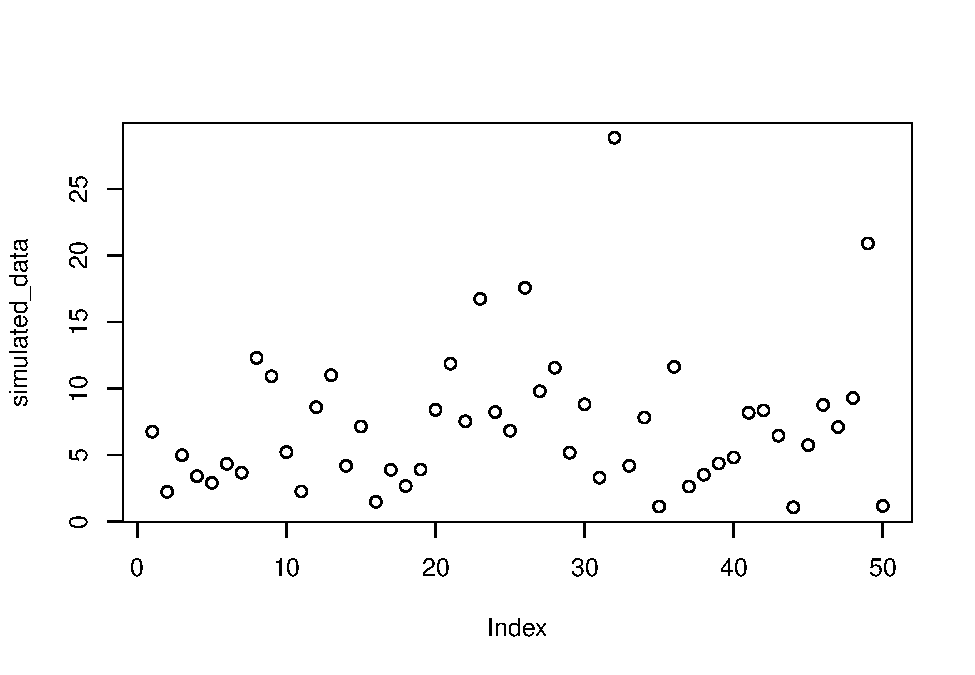
\includegraphics{supplement_files/figure-latex/true-1.pdf}

Next, we generate random starting values for \(a\) and \(b\) for our
chain, taking them from an exponential distribution.

\begin{Shaded}
\begin{Highlighting}[]
\CommentTok{\# rate for exponential distribution}
\NormalTok{alpha }\OtherTok{=} \FloatTok{0.5}

\CommentTok{\# draw 2 values from exponential distribution}
\NormalTok{a }\OtherTok{\textless{}{-}} \FunctionTok{rexp}\NormalTok{(}\DecValTok{1}\NormalTok{, }\DecValTok{1}\SpecialCharTok{/}\NormalTok{alpha)}
\NormalTok{b }\OtherTok{\textless{}{-}} \FunctionTok{rexp}\NormalTok{(}\DecValTok{1}\NormalTok{, }\DecValTok{1}\SpecialCharTok{/}\NormalTok{alpha)}
\end{Highlighting}
\end{Shaded}

We define functions to calculate the likelihood and prior.

\begin{Shaded}
\begin{Highlighting}[]
\CommentTok{\# function to calculate likelihood}
\NormalTok{likelihood }\OtherTok{\textless{}{-}} \ControlFlowTok{function}\NormalTok{(a, b, datos) \{}
    \ControlFlowTok{if}\NormalTok{ ((a }\SpecialCharTok{{-}}\NormalTok{ b) }\SpecialCharTok{\textless{}} \DecValTok{0}\NormalTok{) \{}
\NormalTok{        like }\OtherTok{\textless{}{-}} \DecValTok{0}
        \FunctionTok{return}\NormalTok{(like)  }\CommentTok{\#fail}
\NormalTok{    \} }\ControlFlowTok{else}\NormalTok{ \{}
        \CommentTok{\# product of all vectors of elements in gamma dist}
\NormalTok{        like }\OtherTok{\textless{}{-}} \FunctionTok{prod}\NormalTok{(}\FunctionTok{dgamma}\NormalTok{(datos, }\DecValTok{2}\NormalTok{, }\AttributeTok{rate =}\NormalTok{ (a }\SpecialCharTok{{-}}\NormalTok{ b)))}
        \FunctionTok{return}\NormalTok{(like)}
\NormalTok{    \}}
\NormalTok{\}}

\CommentTok{\# function to calculate prior}
\NormalTok{prior }\OtherTok{\textless{}{-}} \ControlFlowTok{function}\NormalTok{(a, b) \{}
    \ControlFlowTok{if}\NormalTok{ ((a }\SpecialCharTok{{-}}\NormalTok{ b) }\SpecialCharTok{\textless{}} \DecValTok{0}\NormalTok{) \{}
\NormalTok{        prior.val }\OtherTok{\textless{}{-}} \DecValTok{0}
        \FunctionTok{return}\NormalTok{(prior.val)}
\NormalTok{    \} }\ControlFlowTok{else}\NormalTok{ \{}
\NormalTok{        prior.val }\OtherTok{\textless{}{-}} \FunctionTok{dexp}\NormalTok{(a, }\DecValTok{1}\SpecialCharTok{/}\NormalTok{alpha) }\SpecialCharTok{*} \FunctionTok{dexp}\NormalTok{(b, }\DecValTok{1}\SpecialCharTok{/}\NormalTok{alpha)}
        \FunctionTok{return}\NormalTok{(prior.val)}
\NormalTok{    \}}
\NormalTok{\}}
\end{Highlighting}
\end{Shaded}

Then we run an MCMC chain of 5000 generations, logging the results of
the run as it progresses.

\begin{Shaded}
\begin{Highlighting}[]
\CommentTok{\# number of generations to run chain}
\NormalTok{generations }\OtherTok{\textless{}{-}} \DecValTok{5000}

\CommentTok{\# limits on sampling (+ or {-} this value)}
\NormalTok{delta }\OtherTok{\textless{}{-}} \FloatTok{0.25}

\CommentTok{\# prepare output matrix}
\NormalTok{output }\OtherTok{\textless{}{-}} \FunctionTok{matrix}\NormalTok{(}\FunctionTok{rep}\NormalTok{(}\DecValTok{0}\NormalTok{, }\DecValTok{6} \SpecialCharTok{*}\NormalTok{ generations), }\AttributeTok{ncol =} \DecValTok{6}\NormalTok{)}

\ControlFlowTok{for}\NormalTok{ (i }\ControlFlowTok{in} \DecValTok{1}\SpecialCharTok{:}\NormalTok{generations) \{}
    \CommentTok{\# modify params (step)}
\NormalTok{    a\_prime }\OtherTok{\textless{}{-}}\NormalTok{ a }\SpecialCharTok{+} \FunctionTok{runif}\NormalTok{(}\DecValTok{1}\NormalTok{, }\SpecialCharTok{{-}}\NormalTok{delta, delta)}
\NormalTok{    b\_prime }\OtherTok{\textless{}{-}}\NormalTok{ b }\SpecialCharTok{+} \FunctionTok{runif}\NormalTok{(}\DecValTok{1}\NormalTok{, }\SpecialCharTok{{-}}\NormalTok{delta, delta)}

    \CommentTok{\# calculate ratio of likelihoods of new values / old}
    \CommentTok{\# values}
\NormalTok{    like\_odds }\OtherTok{\textless{}{-}} \FunctionTok{likelihood}\NormalTok{(a\_prime, b\_prime, simulated\_data)}\SpecialCharTok{/}\FunctionTok{likelihood}\NormalTok{(a,}
\NormalTok{        b, simulated\_data)}

    \CommentTok{\# calculate ratio of prior of new values / old values}
\NormalTok{    prior\_odds }\OtherTok{\textless{}{-}} \FunctionTok{prior}\NormalTok{(a\_prime, b\_prime)}\SpecialCharTok{/}\FunctionTok{prior}\NormalTok{(a, b)}

    \CommentTok{\# calculate posterior odds}
\NormalTok{    R }\OtherTok{\textless{}{-}}\NormalTok{ like\_odds }\SpecialCharTok{*}\NormalTok{ prior\_odds}

    \CommentTok{\# randomly draw from uniform distribution}
\NormalTok{    u }\OtherTok{\textless{}{-}} \FunctionTok{runif}\NormalTok{(}\DecValTok{1}\NormalTok{)}

    \CommentTok{\# if posterior odds are greater than a random value,}
    \CommentTok{\# keep new values of parameter}
    \ControlFlowTok{if}\NormalTok{ (u }\SpecialCharTok{\textless{}}\NormalTok{ R) \{}
\NormalTok{        a }\OtherTok{=}\NormalTok{ a\_prime}
\NormalTok{        b }\OtherTok{=}\NormalTok{ b\_prime}
\NormalTok{    \}}

    \CommentTok{\# calculate posterior (likelihood*prior)}
\NormalTok{    posterior }\OtherTok{\textless{}{-}} \FunctionTok{likelihood}\NormalTok{(a, b, simulated\_data) }\SpecialCharTok{*} \FunctionTok{prior}\NormalTok{(a,}
\NormalTok{        b)}

    \CommentTok{\# store output}
\NormalTok{    output[i, }\DecValTok{1}\NormalTok{] }\OtherTok{\textless{}{-}}\NormalTok{ i}
\NormalTok{    output[i, }\DecValTok{2}\NormalTok{] }\OtherTok{\textless{}{-}} \FunctionTok{prior}\NormalTok{(a, b)}
\NormalTok{    output[i, }\DecValTok{3}\NormalTok{] }\OtherTok{\textless{}{-}} \FunctionTok{likelihood}\NormalTok{(a, b, simulated\_data)}
\NormalTok{    output[i, }\DecValTok{4}\NormalTok{] }\OtherTok{\textless{}{-}}\NormalTok{ posterior}
\NormalTok{    output[i, }\DecValTok{5}\NormalTok{] }\OtherTok{\textless{}{-}}\NormalTok{ a}
\NormalTok{    output[i, }\DecValTok{6}\NormalTok{] }\OtherTok{\textless{}{-}}\NormalTok{ b}
\NormalTok{\}}

\CommentTok{\# format output data}
\NormalTok{output }\OtherTok{\textless{}{-}} \FunctionTok{data.frame}\NormalTok{(output)}
\FunctionTok{names}\NormalTok{(output) }\OtherTok{\textless{}{-}} \FunctionTok{c}\NormalTok{(}\StringTok{"iteration"}\NormalTok{, }\StringTok{"prior"}\NormalTok{, }\StringTok{"likelihood"}\NormalTok{, }\StringTok{"posterior"}\NormalTok{,}
    \StringTok{"lambda"}\NormalTok{, }\StringTok{"mu"}\NormalTok{)}
\end{Highlighting}
\end{Shaded}

We can then plot the results of our chain. Here we plot the values of
\(a\) and \(b\) over time, showing how they vary dramatically and are
highly correlated. However, when we plot \(a-b\) we find that we are
much better at approximating the value of the difference between these
parameters. Even when \(a\) and \(b\) vary wildly our estimates of
\(a-b\) remain stable.

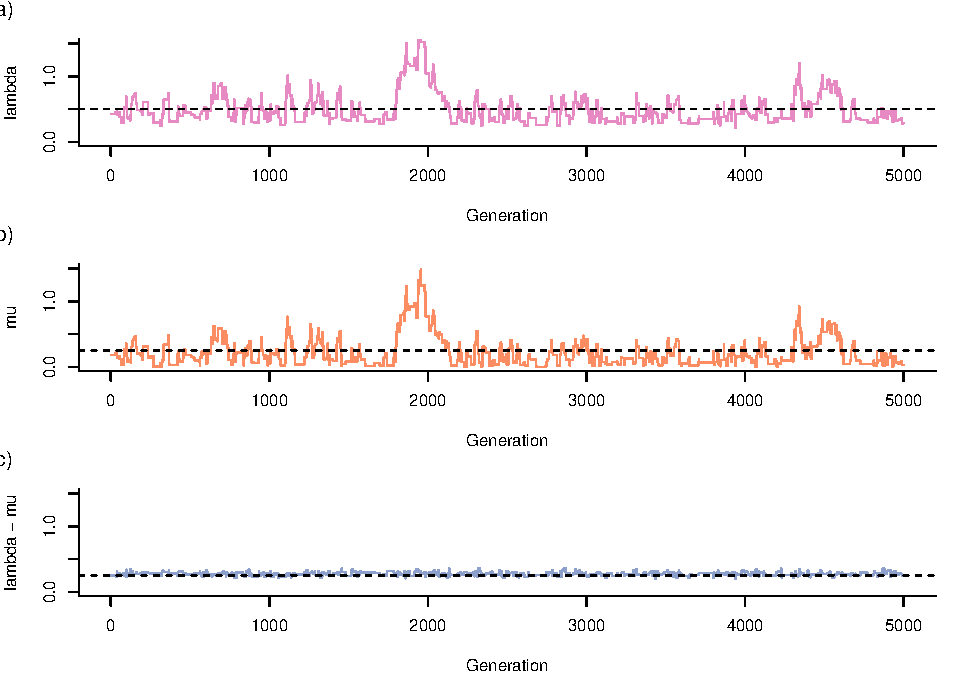
\includegraphics{supplement_files/figure-latex/plot1-1.pdf}

Finally, we plot the relative likelihoods across a range of values we
are interested in for \(a\) and \(b\). We do this by finding the pair of
values for \(a\) and \(b\) that produce the maximum likelihood, and then
divide the likelihood of all other combinations of \(a\) and \(b\) by
the maximum likelihood. This produces a likelihood surface that clearly
shows the high correlation between \(a\) and \(b\), but also that
different pairs of values can be equally likely. The true values of
\(a\) and \(b\) are shown as the orange dot. Even though this falls
within a region of high likelihood as estimated by our model, it
provides no reliable estimate of the absolute values of \(a\) and \(b\)
due to unidentifiability.

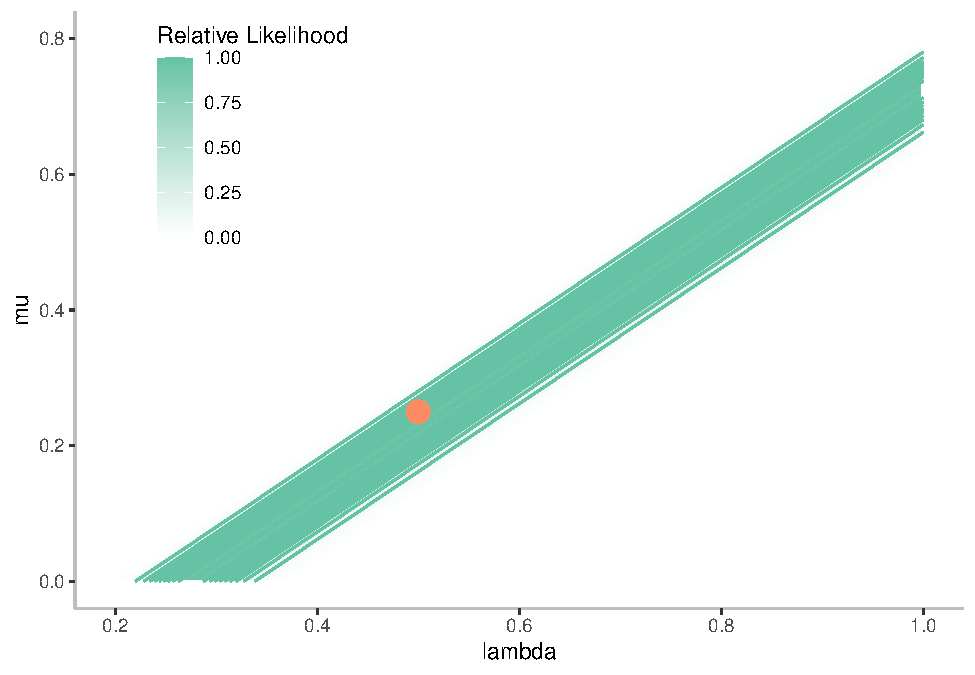
\includegraphics{supplement_files/figure-latex/plot3-1.pdf}

\pagebreak

\hypertarget{section-2-simulations-for-figures-3-and-4}{%
\section{Section 2: Simulations for figures 3 and
4}\label{section-2-simulations-for-figures-3-and-4}}

To construct figures 3 and 4 we first generated values of speciation and
extinction rate over time. In Figure 3 we set speciation rate to be
constant over time. For Figure 4 we used a slightly more complex a
function in which speciation rate increased gradually over time,
centered at 100 Ma, while extinction rate remained constant. With these
known values of speciation and extinction rate we were able to
calculated pulled speciation, diversification and extinction rates using
the equations in Louca \& Pennell, 2020.

We then used our functions of speciation and extinction rates over time
to simulate 50 trees under a birth death model using the function
rbdtree() from the R package `ape'. We generated Lineages-Through-Time
(LTT) plots for the resulting trees (Figs. 3e, 4e) and calculated the
slopes for each LTT using a loess function. We plotted the values of the
slopes at each step (or event) in each LTT to show how the change in
these slopes over time is captured by pulled speciation rate (Figs. 3f,
4f). The initial estimates of slope (Figs. 3f, 4f) can be higher than
the diversification rate as we can only consider scenarios where early
lineages survive. Likewise, the generally wide range of values around
300 Ma is due to a lack of speciation and extinction events leading to a
poor estimation of rates early on. We note that the point estimates of
slope in Figures 3f, 4f are calculated with a sliding window and this
will introduce autocorrelation among estimates.

The github repository \url{https://github.com/ajhelmstetter/pulledRates}
contains the full code for reproducing figures
\href{https://github.com/ajhelmstetter/pulledRates/blob/master/rscripts/fig3.R}{3}
and
\href{https://github.com/ajhelmstetter/pulledRates/blob/master/rscripts/fig4.R}{4}.
This research compendium was made with the help of
\href{https://github.com/FRBCesab/rcompendium}{rcompendium}.

\pagebreak

\hypertarget{section-3-how-does-variation-in-r-affect-r_p}{%
\section{\texorpdfstring{Section 3: How does variation in \(r\) affect
\(r_p\)
?}{Section 3: How does variation in r affect r\_p ?}}\label{section-3-how-does-variation-in-r-affect-r_p}}

\hypertarget{preliminary-functions}{%
\subsection{Preliminary functions}\label{preliminary-functions}}

The following function returns the three pulled rates. Arguments are the
birth and death rates (functions), the sampling fraction (real number)
and a time series for integration.

\begin{Shaded}
\begin{Highlighting}[]
\NormalTok{pulled }\OtherTok{\textless{}{-}} \ControlFlowTok{function}\NormalTok{(birth, death, rho, t) \{}
\NormalTok{    params }\OtherTok{\textless{}{-}} \FunctionTok{numeric}\NormalTok{(}\DecValTok{0}\NormalTok{)}
    \CommentTok{\# The following function is passed to the R function}
    \CommentTok{\# ode()}
\NormalTok{    fn }\OtherTok{\textless{}{-}} \ControlFlowTok{function}\NormalTok{(t, e, params) \{}
        \FunctionTok{with}\NormalTok{(}\FunctionTok{as.list}\NormalTok{(}\FunctionTok{c}\NormalTok{(e, params)), \{}
\NormalTok{            g }\OtherTok{\textless{}{-}} \FunctionTok{death}\NormalTok{(t) }\SpecialCharTok{{-}}\NormalTok{ e }\SpecialCharTok{*}\NormalTok{ (}\FunctionTok{birth}\NormalTok{(t) }\SpecialCharTok{+} \FunctionTok{death}\NormalTok{(t)) }\SpecialCharTok{+}\NormalTok{ e }\SpecialCharTok{*}\NormalTok{ e }\SpecialCharTok{*}
                \FunctionTok{birth}\NormalTok{(t)}
            \FunctionTok{return}\NormalTok{(}\FunctionTok{list}\NormalTok{(g))}
\NormalTok{        \})}
\NormalTok{    \}}
\NormalTok{    E0 }\OtherTok{\textless{}{-}} \DecValTok{1} \SpecialCharTok{{-}}\NormalTok{ rho  }\CommentTok{\# initial value for E}
\NormalTok{    Enum }\OtherTok{\textless{}{-}} \FunctionTok{ode}\NormalTok{(E0, t, fn, params)  }\CommentTok{\# Numerical integration of e}
\NormalTok{    PSRfull }\OtherTok{\textless{}{-}} \FunctionTok{birth}\NormalTok{(t) }\SpecialCharTok{*}\NormalTok{ (}\DecValTok{1} \SpecialCharTok{{-}}\NormalTok{ Enum[, }\DecValTok{2}\NormalTok{])  }\CommentTok{\# Pulled speciation rate}
    \CommentTok{\# To get all vectors with the same length we suppress}
    \CommentTok{\# the last value of the vector because only intervals}
    \CommentTok{\# are considered for the derivative}
\NormalTok{    PSR }\OtherTok{\textless{}{-}}\NormalTok{ PSRfull[}\SpecialCharTok{{-}}\FunctionTok{length}\NormalTok{(PSRfull)]}
\NormalTok{    tt }\OtherTok{\textless{}{-}}\NormalTok{ t[}\SpecialCharTok{{-}}\FunctionTok{length}\NormalTok{(t)]}
\NormalTok{    dt }\OtherTok{\textless{}{-}}\NormalTok{ t[}\DecValTok{2}\NormalTok{] }\SpecialCharTok{{-}}\NormalTok{ t[}\DecValTok{1}\NormalTok{]  }\CommentTok{\# to get the time interval}
\NormalTok{    PDR }\OtherTok{\textless{}{-}} \FunctionTok{birth}\NormalTok{(tt) }\SpecialCharTok{{-}} \FunctionTok{death}\NormalTok{(tt) }\SpecialCharTok{+} \FunctionTok{diff}\NormalTok{(}\FunctionTok{birth}\NormalTok{(t))}\SpecialCharTok{/}\NormalTok{(dt }\SpecialCharTok{*} \FunctionTok{birth}\NormalTok{(tt))  }\CommentTok{\# Pulled diversification rate}
\NormalTok{    PER }\OtherTok{\textless{}{-}} \FunctionTok{birth}\NormalTok{(}\DecValTok{0}\NormalTok{)}\SpecialCharTok{/}\NormalTok{(}\DecValTok{1} \SpecialCharTok{{-}}\NormalTok{ E0) }\SpecialCharTok{{-}}\NormalTok{ PDR  }\CommentTok{\# Pulled extinction rate}
    \FunctionTok{return}\NormalTok{(}\FunctionTok{list}\NormalTok{(}\AttributeTok{PSR =}\NormalTok{ PSR, }\AttributeTok{PER =}\NormalTok{ PER, }\AttributeTok{PDR =}\NormalTok{ PDR))}
\NormalTok{\}}
\end{Highlighting}
\end{Shaded}

A function to do more or less sharp but continuous shifts in rates
between rates `r0' and `r1'. `Tshift' is the timing of the shft and
`alpha' controls the sharpness of the shift (where increasing values are
sharper).

\begin{Shaded}
\begin{Highlighting}[]
\NormalTok{smooth\_stepwise }\OtherTok{\textless{}{-}} \ControlFlowTok{function}\NormalTok{(r0, r1, Tshift, alpha, t) \{}
\NormalTok{    (r0 }\SpecialCharTok{*} \FunctionTok{exp}\NormalTok{(alpha }\SpecialCharTok{*}\NormalTok{ (t }\SpecialCharTok{{-}}\NormalTok{ Tshift)) }\SpecialCharTok{+}\NormalTok{ r1)}\SpecialCharTok{/}\NormalTok{(}\FunctionTok{exp}\NormalTok{(alpha }\SpecialCharTok{*}\NormalTok{ (t }\SpecialCharTok{{-}}\NormalTok{ Tshift)) }\SpecialCharTok{+}
        \DecValTok{1}\NormalTok{)}
\NormalTok{\}}
\end{Highlighting}
\end{Shaded}

\pagebreak

A function to generate four figures for a given scenario. `spe' and
`ext' are functions for speciation and extinction rate through time, and
`rho' is the sampling fraction. `seq\_time' is a vector of time
intervals.

\begin{Shaded}
\begin{Highlighting}[]
\NormalTok{plot\_scenario }\OtherTok{\textless{}{-}} \ControlFlowTok{function}\NormalTok{(spe, ext, rho, seq\_time) \{}

\NormalTok{    pulled\_rates }\OtherTok{\textless{}{-}} \FunctionTok{pulled}\NormalTok{(}\AttributeTok{birth =}\NormalTok{ spe, }\AttributeTok{death =}\NormalTok{ ext, }\AttributeTok{rho =}\NormalTok{ rho,}
        \AttributeTok{t =}\NormalTok{ seq\_time)}
\NormalTok{    div }\OtherTok{\textless{}{-}} \ControlFlowTok{function}\NormalTok{(x) }\FunctionTok{spe}\NormalTok{(x) }\SpecialCharTok{{-}} \FunctionTok{ext}\NormalTok{(x)}
\NormalTok{    PSR }\OtherTok{\textless{}{-}}\NormalTok{ pulled\_rates}\SpecialCharTok{$}\NormalTok{PSR}
\NormalTok{    PER }\OtherTok{\textless{}{-}}\NormalTok{ pulled\_rates}\SpecialCharTok{$}\NormalTok{PER}
\NormalTok{    PDR }\OtherTok{\textless{}{-}}\NormalTok{ pulled\_rates}\SpecialCharTok{$}\NormalTok{PDR}

    \CommentTok{\# remove last time value to match differences / pulled}
    \CommentTok{\# rates}
\NormalTok{    t }\OtherTok{\textless{}{-}}\NormalTok{ seq\_time[}\SpecialCharTok{{-}}\FunctionTok{length}\NormalTok{(seq\_time)]}

    \CommentTok{\# layout}
    \FunctionTok{par}\NormalTok{(}\AttributeTok{mar =} \FunctionTok{c}\NormalTok{(}\DecValTok{4}\NormalTok{, }\DecValTok{2}\NormalTok{, }\DecValTok{1}\NormalTok{, }\DecValTok{1}\NormalTok{))}
    \FunctionTok{par}\NormalTok{(}\AttributeTok{mfrow =} \FunctionTok{c}\NormalTok{(}\DecValTok{2}\NormalTok{, }\DecValTok{2}\NormalTok{))}
    \FunctionTok{palette}\NormalTok{(}\FunctionTok{alpha}\NormalTok{(}\FunctionTok{brewer.pal}\NormalTok{(}\DecValTok{5}\NormalTok{, }\StringTok{"Set1"}\NormalTok{), }\FloatTok{0.75}\NormalTok{))}

    \CommentTok{\# True rates}

    \CommentTok{\# set y axis values based on rates Ymin \textless{}{-}}
    \CommentTok{\# 0.9*min(rev(spe(t)), rev(ext(t)),rev(div(t))) {-} 0.03}
    \CommentTok{\# Ymax \textless{}{-} 1.1*max(rev(spe(t)), rev(ext(t)),rev(div(t)))}
    \CommentTok{\# + 0.06}

    \CommentTok{\# fixed y axis values}
\NormalTok{    Ymin }\OtherTok{\textless{}{-}} \SpecialCharTok{{-}}\FloatTok{0.1}
\NormalTok{    Ymax }\OtherTok{\textless{}{-}} \FloatTok{0.25}

    \FunctionTok{plot}\NormalTok{(}\FunctionTok{rev}\NormalTok{(}\FunctionTok{spe}\NormalTok{(t)) }\SpecialCharTok{\textasciitilde{}} \FunctionTok{rev}\NormalTok{(}\SpecialCharTok{{-}}\NormalTok{t), }\AttributeTok{type =} \StringTok{"l"}\NormalTok{, }\AttributeTok{col =} \DecValTok{2}\NormalTok{, }\AttributeTok{ylim =} \FunctionTok{c}\NormalTok{(Ymin,}
\NormalTok{        Ymax), }\AttributeTok{ylab =} \StringTok{""}\NormalTok{, }\AttributeTok{cex.lab =} \FloatTok{0.75}\NormalTok{, }\AttributeTok{cex.axis =} \FloatTok{0.75}\NormalTok{, }\AttributeTok{xlab =} \FunctionTok{bquote}\NormalTok{(}\StringTok{"Age ("} \SpecialCharTok{*}
\NormalTok{        tau }\SpecialCharTok{*} \StringTok{")"}\NormalTok{), }\AttributeTok{xaxt =} \StringTok{"n"}\NormalTok{)}
    \FunctionTok{axis}\NormalTok{(}\DecValTok{1}\NormalTok{, }\AttributeTok{at =} \FunctionTok{pretty}\NormalTok{(}\FunctionTok{range}\NormalTok{(}\FunctionTok{rev}\NormalTok{(}\SpecialCharTok{{-}}\NormalTok{t))), }\AttributeTok{labels =} \FunctionTok{rev}\NormalTok{(}\FunctionTok{pretty}\NormalTok{(}\FunctionTok{range}\NormalTok{(}\FunctionTok{rev}\NormalTok{(t)))),}
        \AttributeTok{cex.axis =} \FloatTok{0.75}\NormalTok{)}
    \FunctionTok{lines}\NormalTok{(}\FunctionTok{rev}\NormalTok{(}\FunctionTok{ext}\NormalTok{(t)) }\SpecialCharTok{\textasciitilde{}} \FunctionTok{rev}\NormalTok{(}\SpecialCharTok{{-}}\NormalTok{t), }\AttributeTok{col =} \DecValTok{1}\NormalTok{)}
    \FunctionTok{lines}\NormalTok{(}\FunctionTok{rev}\NormalTok{(}\FunctionTok{div}\NormalTok{(t)) }\SpecialCharTok{\textasciitilde{}} \FunctionTok{rev}\NormalTok{(}\SpecialCharTok{{-}}\NormalTok{t), }\AttributeTok{col =} \StringTok{"black"}\NormalTok{)}
    \FunctionTok{legend}\NormalTok{(}\StringTok{"topright"}\NormalTok{, }\AttributeTok{legend =} \FunctionTok{c}\NormalTok{(}\StringTok{"speciation rate"}\NormalTok{, }\StringTok{"extinction rate"}\NormalTok{,}
        \StringTok{"diversification rate"}\NormalTok{), }\AttributeTok{lty =} \DecValTok{1}\NormalTok{, }\AttributeTok{col =} \FunctionTok{c}\NormalTok{(}\DecValTok{2}\NormalTok{, }\DecValTok{1}\NormalTok{, }\StringTok{"black"}\NormalTok{),}
        \AttributeTok{bty =} \StringTok{"n"}\NormalTok{, }\AttributeTok{cex =} \FloatTok{0.5}\NormalTok{)}

    \CommentTok{\# True and pulled diversification rates Ymin \textless{}{-}}
    \CommentTok{\# 0.9*min(rev(div(t)), PDR) {-} 0.03 Ymax \textless{}{-}}
    \CommentTok{\# 1.1*max(rev(div(t)), PDR) + 0.06}
    \FunctionTok{plot}\NormalTok{(}\FunctionTok{rev}\NormalTok{(}\FunctionTok{div}\NormalTok{(t)) }\SpecialCharTok{\textasciitilde{}} \FunctionTok{rev}\NormalTok{(}\SpecialCharTok{{-}}\NormalTok{t), }\AttributeTok{type =} \StringTok{"l"}\NormalTok{, }\AttributeTok{col =} \StringTok{"black"}\NormalTok{, }\AttributeTok{ylim =} \FunctionTok{c}\NormalTok{(Ymin,}
\NormalTok{        Ymax), }\AttributeTok{ylab =} \StringTok{""}\NormalTok{, }\AttributeTok{cex.lab =} \FloatTok{0.75}\NormalTok{, }\AttributeTok{cex.axis =} \FloatTok{0.75}\NormalTok{, }\AttributeTok{xlab =} \FunctionTok{bquote}\NormalTok{(}\StringTok{"Age ("} \SpecialCharTok{*}
\NormalTok{        tau }\SpecialCharTok{*} \StringTok{")"}\NormalTok{), }\AttributeTok{xaxt =} \StringTok{"n"}\NormalTok{)}
    \FunctionTok{axis}\NormalTok{(}\DecValTok{1}\NormalTok{, }\AttributeTok{at =} \FunctionTok{pretty}\NormalTok{(}\FunctionTok{range}\NormalTok{(}\FunctionTok{rev}\NormalTok{(}\SpecialCharTok{{-}}\NormalTok{t))), }\AttributeTok{labels =} \FunctionTok{rev}\NormalTok{(}\FunctionTok{pretty}\NormalTok{(}\FunctionTok{range}\NormalTok{(}\FunctionTok{rev}\NormalTok{(t)))),}
        \AttributeTok{cex.axis =} \FloatTok{0.75}\NormalTok{)}
    \FunctionTok{lines}\NormalTok{(}\FunctionTok{rev}\NormalTok{(PDR) }\SpecialCharTok{\textasciitilde{}} \FunctionTok{rev}\NormalTok{(}\SpecialCharTok{{-}}\NormalTok{t), }\AttributeTok{col =} \StringTok{"black"}\NormalTok{, }\AttributeTok{lty =} \DecValTok{2}\NormalTok{)}
    \FunctionTok{legend}\NormalTok{(}\StringTok{"topright"}\NormalTok{, }\AttributeTok{legend =} \FunctionTok{c}\NormalTok{(}\StringTok{"diversification rate"}\NormalTok{, }\StringTok{"pulled diversification rate"}\NormalTok{),}
        \AttributeTok{lty =} \FunctionTok{c}\NormalTok{(}\DecValTok{1}\NormalTok{, }\DecValTok{2}\NormalTok{), }\AttributeTok{col =} \FunctionTok{c}\NormalTok{(}\StringTok{"black"}\NormalTok{), }\AttributeTok{bty =} \StringTok{"n"}\NormalTok{, }\AttributeTok{cex =} \FloatTok{0.5}\NormalTok{)}

    \CommentTok{\# True and pulled speciation and extinction rates Ymin}
    \CommentTok{\# \textless{}{-} 0.9*min(rev(spe(t)), PSR,rev(ext(t))) {-} 0.03 Ymax}
    \CommentTok{\# \textless{}{-} 1.1*max(rev(spe(t)), PSR,rev(ext(t))) + 0.06}
    \FunctionTok{plot}\NormalTok{(}\FunctionTok{rev}\NormalTok{(}\FunctionTok{spe}\NormalTok{(t)) }\SpecialCharTok{\textasciitilde{}} \FunctionTok{rev}\NormalTok{(}\SpecialCharTok{{-}}\NormalTok{t), }\AttributeTok{type =} \StringTok{"l"}\NormalTok{, }\AttributeTok{col =} \DecValTok{2}\NormalTok{, }\AttributeTok{ylim =} \FunctionTok{c}\NormalTok{(Ymin,}
\NormalTok{        Ymax), }\AttributeTok{ylab =} \StringTok{""}\NormalTok{, }\AttributeTok{cex.lab =} \FloatTok{0.75}\NormalTok{, }\AttributeTok{cex.axis =} \FloatTok{0.75}\NormalTok{, }\AttributeTok{xlab =} \FunctionTok{bquote}\NormalTok{(}\StringTok{"Age ("} \SpecialCharTok{*}
\NormalTok{        tau }\SpecialCharTok{*} \StringTok{")"}\NormalTok{), }\AttributeTok{xaxt =} \StringTok{"n"}\NormalTok{)}
    \FunctionTok{axis}\NormalTok{(}\DecValTok{1}\NormalTok{, }\AttributeTok{at =} \FunctionTok{pretty}\NormalTok{(}\FunctionTok{range}\NormalTok{(}\FunctionTok{rev}\NormalTok{(}\SpecialCharTok{{-}}\NormalTok{t))), }\AttributeTok{labels =} \FunctionTok{rev}\NormalTok{(}\FunctionTok{pretty}\NormalTok{(}\FunctionTok{range}\NormalTok{(}\FunctionTok{rev}\NormalTok{(t)))),}
        \AttributeTok{cex.axis =} \FloatTok{0.75}\NormalTok{)}
    \FunctionTok{lines}\NormalTok{(}\FunctionTok{rev}\NormalTok{(PSR) }\SpecialCharTok{\textasciitilde{}} \FunctionTok{rev}\NormalTok{(}\SpecialCharTok{{-}}\NormalTok{t), }\AttributeTok{col =} \DecValTok{2}\NormalTok{, }\AttributeTok{lty =} \DecValTok{2}\NormalTok{)}
    \FunctionTok{lines}\NormalTok{(}\FunctionTok{rev}\NormalTok{(}\FunctionTok{ext}\NormalTok{(t)) }\SpecialCharTok{\textasciitilde{}} \FunctionTok{rev}\NormalTok{(}\SpecialCharTok{{-}}\NormalTok{t), }\AttributeTok{type =} \StringTok{"l"}\NormalTok{, }\AttributeTok{col =} \DecValTok{1}\NormalTok{)}
    \FunctionTok{lines}\NormalTok{(}\FunctionTok{rev}\NormalTok{(PER) }\SpecialCharTok{\textasciitilde{}} \FunctionTok{rev}\NormalTok{(}\SpecialCharTok{{-}}\NormalTok{t), }\AttributeTok{col =} \DecValTok{1}\NormalTok{, }\AttributeTok{lty =} \DecValTok{2}\NormalTok{)}
    \FunctionTok{legend}\NormalTok{(}\StringTok{"topright"}\NormalTok{, }\AttributeTok{legend =} \FunctionTok{c}\NormalTok{(}\StringTok{"speciation rate"}\NormalTok{, }\StringTok{"pulled speciation rate"}\NormalTok{,}
        \StringTok{"extinction rate"}\NormalTok{, }\StringTok{"pulled extinction rate"}\NormalTok{), }\AttributeTok{lty =} \FunctionTok{c}\NormalTok{(}\DecValTok{1}\NormalTok{,}
        \DecValTok{2}\NormalTok{, }\DecValTok{1}\NormalTok{, }\DecValTok{2}\NormalTok{), }\AttributeTok{col =} \FunctionTok{c}\NormalTok{(}\DecValTok{2}\NormalTok{, }\DecValTok{2}\NormalTok{, }\DecValTok{1}\NormalTok{, }\DecValTok{1}\NormalTok{), }\AttributeTok{bty =} \StringTok{"n"}\NormalTok{, }\AttributeTok{cex =} \FloatTok{0.5}\NormalTok{)}

    \CommentTok{\# Pulled rates Ymin \textless{}{-} 0.9*min(PSR, PDR) {-} 0.03 Ymax \textless{}{-}}
    \CommentTok{\# 1.1*max(PSR, PDR) + 0.06}
    \FunctionTok{plot}\NormalTok{(}\FunctionTok{rev}\NormalTok{(PDR) }\SpecialCharTok{\textasciitilde{}} \FunctionTok{rev}\NormalTok{(}\SpecialCharTok{{-}}\NormalTok{t), }\AttributeTok{type =} \StringTok{"l"}\NormalTok{, }\AttributeTok{lty =} \DecValTok{2}\NormalTok{, }\AttributeTok{col =} \StringTok{"black"}\NormalTok{,}
        \AttributeTok{ylim =} \FunctionTok{c}\NormalTok{(Ymin, Ymax), }\AttributeTok{ylab =} \StringTok{""}\NormalTok{, }\AttributeTok{cex.lab =} \FloatTok{0.75}\NormalTok{, }\AttributeTok{cex.axis =} \FloatTok{0.75}\NormalTok{,}
        \AttributeTok{xlab =} \FunctionTok{bquote}\NormalTok{(}\StringTok{"Age ("} \SpecialCharTok{*}\NormalTok{ tau }\SpecialCharTok{*} \StringTok{")"}\NormalTok{), }\AttributeTok{xaxt =} \StringTok{"n"}\NormalTok{)}
    \FunctionTok{axis}\NormalTok{(}\DecValTok{1}\NormalTok{, }\AttributeTok{at =} \FunctionTok{pretty}\NormalTok{(}\FunctionTok{range}\NormalTok{(}\FunctionTok{rev}\NormalTok{(}\SpecialCharTok{{-}}\NormalTok{t))), }\AttributeTok{labels =} \FunctionTok{rev}\NormalTok{(}\FunctionTok{pretty}\NormalTok{(}\FunctionTok{range}\NormalTok{(}\FunctionTok{rev}\NormalTok{(t)))),}
        \AttributeTok{cex.axis =} \FloatTok{0.75}\NormalTok{)}
    \FunctionTok{lines}\NormalTok{(}\FunctionTok{rev}\NormalTok{(PSR) }\SpecialCharTok{\textasciitilde{}} \FunctionTok{rev}\NormalTok{(}\SpecialCharTok{{-}}\NormalTok{t), }\AttributeTok{col =} \DecValTok{2}\NormalTok{, }\AttributeTok{lty =} \DecValTok{2}\NormalTok{)}
    \FunctionTok{legend}\NormalTok{(}\StringTok{"topright"}\NormalTok{, }\AttributeTok{legend =} \FunctionTok{c}\NormalTok{(}\StringTok{"pulled speciation rate"}\NormalTok{, }\StringTok{"pulled diversification rate"}\NormalTok{),}
        \AttributeTok{lty =} \FunctionTok{c}\NormalTok{(}\DecValTok{2}\NormalTok{), }\AttributeTok{col =} \FunctionTok{c}\NormalTok{(}\DecValTok{2}\NormalTok{, }\StringTok{"black"}\NormalTok{), }\AttributeTok{bty =} \StringTok{"n"}\NormalTok{, }\AttributeTok{cex =} \FloatTok{0.5}\NormalTok{)}

\NormalTok{\}}
\end{Highlighting}
\end{Shaded}

\pagebreak

\hypertarget{r_p-is-a-generally-a-good-approximation-of-r}{%
\subsection{\texorpdfstring{\(r_p\) is a generally a good approximation
of
\(r\)}{r\_p is a generally a good approximation of r}}\label{r_p-is-a-generally-a-good-approximation-of-r}}

The exploration of the following scenarios demonstrates that even when
\(\lambda_p\) and \(\mu_p\) are very different from \(\lambda\) and
\(\mu\) (as shown in LP), in most cases, \(r\) and \(r_p\) are close. In
the main text, we suggested that when \(r_p\) and \(\lambda_p\) are
quite close (except for recent times), it is a good diagnostic of the
fact that \(\lambda\) does not change too rapidly so that \(r_p\) is a
good proxy for \(r\). The following exploration shows that this
guideline is conservative as even when \(r_p\) and \(\lambda_p\)
substantially differ, \(r_p\) can still be close to \(r\).

For simplicity, the sampling fraction is assumed to be 1 to focus on the
effect of varying extinction and speciation rates, which is what we are
interested in from a biological point of view. The effect of the
sampling fraction can easily be explored by passing rho value to the
pulled() function.

Here we give several examples to illustrate different possible
scenarios. Using this script, any function for the speciation and
extinction rate can be given to play with.

\hypertarget{the-simplest-scenario---constant-rates.}{%
\subsection{The simplest scenario - constant
rates.}\label{the-simplest-scenario---constant-rates.}}

Here speciation and extinction rates are different, but constant over
time. A lack of variation in speciation rate means that \(r_p\) and
\(r\) are the same.

\begin{Shaded}
\begin{Highlighting}[]
\NormalTok{tmax }\OtherTok{\textless{}{-}} \DecValTok{300}
\NormalTok{seq\_time }\OtherTok{\textless{}{-}} \FunctionTok{seq}\NormalTok{(}\DecValTok{0}\NormalTok{, tmax, }\FloatTok{0.1}\NormalTok{)}
\NormalTok{spe0 }\OtherTok{\textless{}{-}} \ControlFlowTok{function}\NormalTok{(x) }\FloatTok{0.05} \SpecialCharTok{+}\NormalTok{ x }\SpecialCharTok{{-}}\NormalTok{ x}
\NormalTok{ext0 }\OtherTok{\textless{}{-}} \ControlFlowTok{function}\NormalTok{(x) }\FloatTok{0.04} \SpecialCharTok{+}\NormalTok{ x }\SpecialCharTok{{-}}\NormalTok{ x}
\FunctionTok{plot\_scenario}\NormalTok{(}\AttributeTok{spe =}\NormalTok{ spe0, }\AttributeTok{ext =}\NormalTok{ ext0, }\AttributeTok{rho =} \DecValTok{1}\NormalTok{, }\AttributeTok{seq\_time =} \FunctionTok{seq}\NormalTok{(}\DecValTok{0}\NormalTok{,}
\NormalTok{    tmax, }\FloatTok{0.1}\NormalTok{))}
\end{Highlighting}
\end{Shaded}

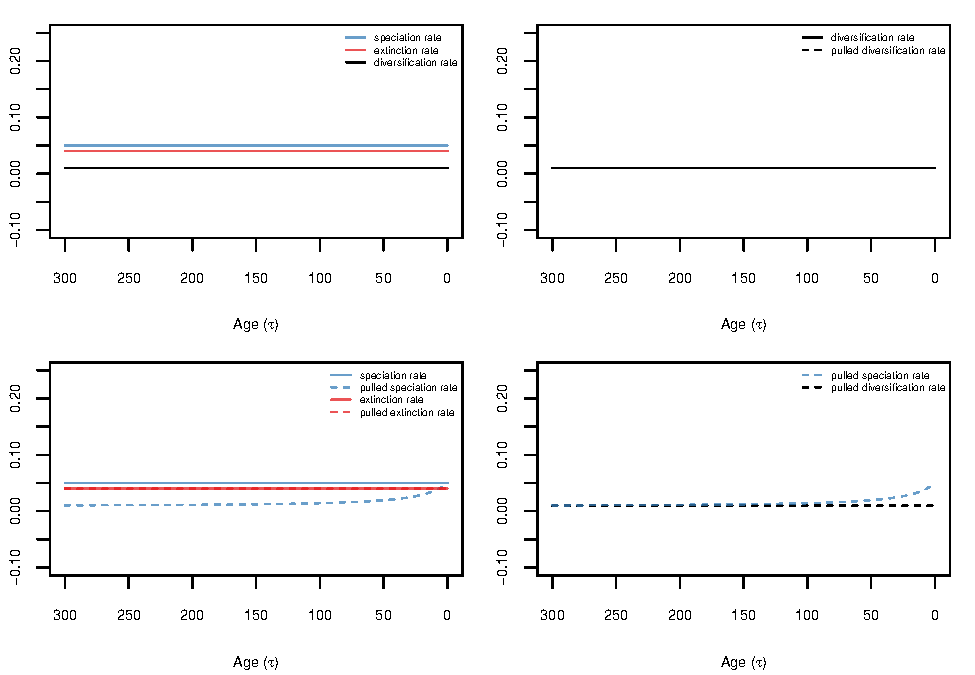
\includegraphics{supplement_files/figure-latex/unnamed-chunk-5-1.pdf}

\pagebreak

\hypertarget{a-single-change-in-speciation-rate}{%
\subsection{A single change in speciation
rate}\label{a-single-change-in-speciation-rate}}

Here we use a stepwise change in speciation rate at 100 Ma with a
smoothing function. When the change in speciation rates is gradual the
true and pulled diversification rate remain quite close.

\begin{Shaded}
\begin{Highlighting}[]
\NormalTok{tmax }\OtherTok{\textless{}{-}} \DecValTok{300}
\NormalTok{seq\_time }\OtherTok{\textless{}{-}} \FunctionTok{seq}\NormalTok{(}\DecValTok{0}\NormalTok{, tmax, }\FloatTok{0.1}\NormalTok{)}
\NormalTok{spe1 }\OtherTok{\textless{}{-}} \ControlFlowTok{function}\NormalTok{(x) }\FunctionTok{smooth\_stepwise}\NormalTok{(}\AttributeTok{r0 =} \FloatTok{0.03}\NormalTok{, }\AttributeTok{r1 =} \FloatTok{0.05}\NormalTok{, }\AttributeTok{Tshift =} \DecValTok{100}\NormalTok{,}
    \AttributeTok{alpha =} \FloatTok{0.05}\NormalTok{, x)}
\NormalTok{ext1 }\OtherTok{\textless{}{-}} \ControlFlowTok{function}\NormalTok{(x) }\FloatTok{0.02} \SpecialCharTok{+}\NormalTok{ x }\SpecialCharTok{{-}}\NormalTok{ x}
\FunctionTok{plot\_scenario}\NormalTok{(}\AttributeTok{spe =}\NormalTok{ spe1, }\AttributeTok{ext =}\NormalTok{ ext1, }\AttributeTok{rho =} \DecValTok{1}\NormalTok{, }\AttributeTok{seq\_time =} \FunctionTok{seq}\NormalTok{(}\DecValTok{0}\NormalTok{,}
\NormalTok{    tmax, }\FloatTok{0.1}\NormalTok{))}
\end{Highlighting}
\end{Shaded}

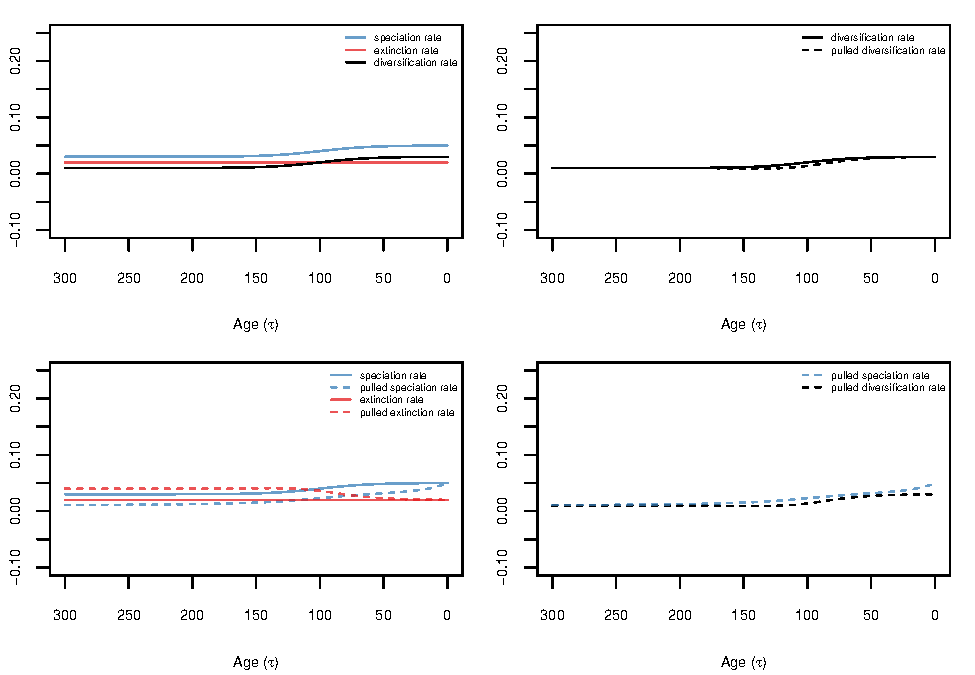
\includegraphics{supplement_files/figure-latex/unnamed-chunk-6-1.pdf}

\pagebreak

Then we looked at a more rapid change. In this case, \(r_p\) strongly
differs from \(r\) but only during a very short period of time, which
would be hard to detect with empirical data.

\begin{Shaded}
\begin{Highlighting}[]
\NormalTok{tmax }\OtherTok{\textless{}{-}} \DecValTok{300}
\NormalTok{seq\_time }\OtherTok{\textless{}{-}} \FunctionTok{seq}\NormalTok{(}\DecValTok{0}\NormalTok{, tmax, }\FloatTok{0.1}\NormalTok{)}
\NormalTok{spe1 }\OtherTok{\textless{}{-}} \ControlFlowTok{function}\NormalTok{(x) }\FunctionTok{smooth\_stepwise}\NormalTok{(}\AttributeTok{r0 =} \FloatTok{0.03}\NormalTok{, }\AttributeTok{r1 =} \FloatTok{0.05}\NormalTok{, }\AttributeTok{Tshift =} \DecValTok{100}\NormalTok{,}
    \AttributeTok{alpha =} \DecValTok{1}\NormalTok{, x)}
\NormalTok{ext1 }\OtherTok{\textless{}{-}} \ControlFlowTok{function}\NormalTok{(x) }\FloatTok{0.02} \SpecialCharTok{+}\NormalTok{ x }\SpecialCharTok{{-}}\NormalTok{ x}
\FunctionTok{plot\_scenario}\NormalTok{(}\AttributeTok{spe =}\NormalTok{ spe1, }\AttributeTok{ext =}\NormalTok{ ext1, }\AttributeTok{rho =} \DecValTok{1}\NormalTok{, }\AttributeTok{seq\_time =} \FunctionTok{seq}\NormalTok{(}\DecValTok{0}\NormalTok{,}
\NormalTok{    tmax, }\FloatTok{0.1}\NormalTok{))}
\end{Highlighting}
\end{Shaded}

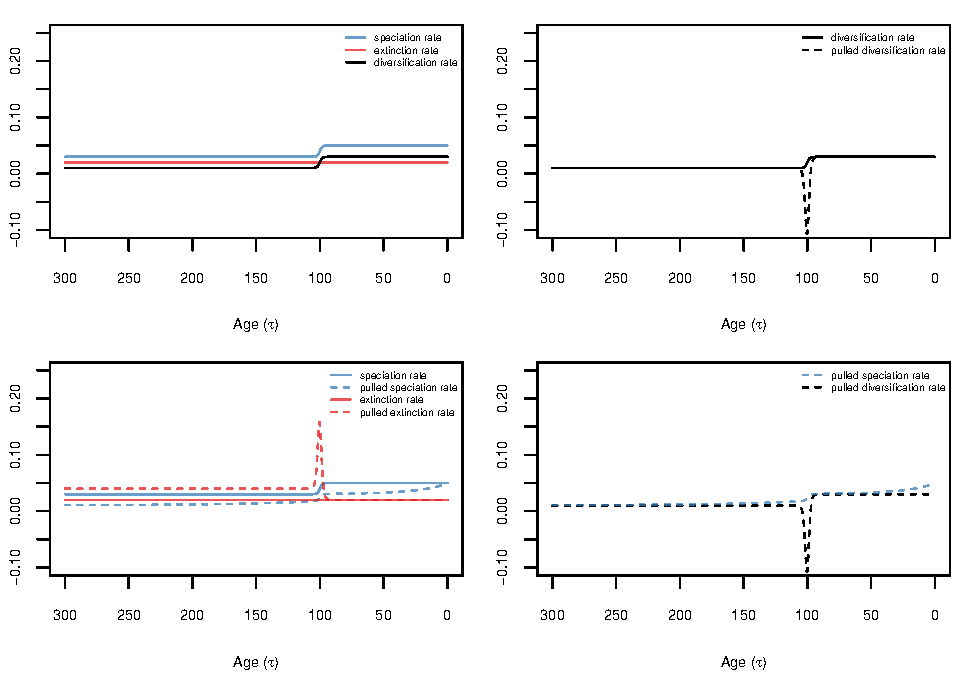
\includegraphics{supplement_files/figure-latex/unnamed-chunk-7-1.pdf}

\pagebreak

\hypertarget{a-single-change-in-extinction-rate}{%
\subsection{A single change in extinction
rate}\label{a-single-change-in-extinction-rate}}

The following two examples are similar to those above but with a shift
in extinction rate. As \(\lambda\) is kept constant, \(r_p = r\), but an
effect is still seen in \(\lambda_p\). First, we show a slow shift.

\begin{Shaded}
\begin{Highlighting}[]
\NormalTok{tmax }\OtherTok{\textless{}{-}} \DecValTok{300}
\NormalTok{seq\_time }\OtherTok{\textless{}{-}} \FunctionTok{seq}\NormalTok{(}\DecValTok{0}\NormalTok{, tmax, }\FloatTok{0.1}\NormalTok{)}
\NormalTok{spe1 }\OtherTok{\textless{}{-}} \ControlFlowTok{function}\NormalTok{(x) }\FloatTok{0.1} \SpecialCharTok{+}\NormalTok{ x }\SpecialCharTok{{-}}\NormalTok{ x}
\NormalTok{ext1 }\OtherTok{\textless{}{-}} \ControlFlowTok{function}\NormalTok{(x) }\FunctionTok{smooth\_stepwise}\NormalTok{(}\AttributeTok{r0 =} \FloatTok{0.02}\NormalTok{, }\AttributeTok{r1 =} \FloatTok{0.045}\NormalTok{, }\AttributeTok{Tshift =} \DecValTok{100}\NormalTok{,}
    \AttributeTok{alpha =} \FloatTok{0.05}\NormalTok{, x)}
\FunctionTok{plot\_scenario}\NormalTok{(}\AttributeTok{spe =}\NormalTok{ spe1, }\AttributeTok{ext =}\NormalTok{ ext1, }\AttributeTok{rho =} \DecValTok{1}\NormalTok{, }\AttributeTok{seq\_time =} \FunctionTok{seq}\NormalTok{(}\DecValTok{0}\NormalTok{,}
\NormalTok{    tmax, }\FloatTok{0.1}\NormalTok{))}
\end{Highlighting}
\end{Shaded}

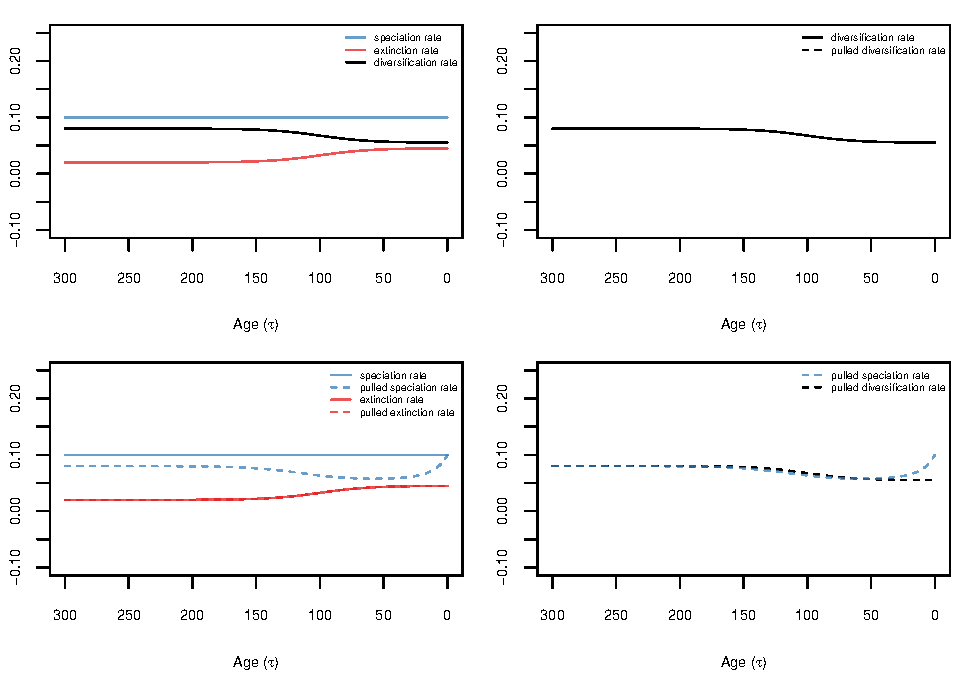
\includegraphics{supplement_files/figure-latex/unnamed-chunk-8-1.pdf}

\pagebreak

Second, a rapid shift in extinction rate causing \(\lambda_p\) to depart
from \(r_p\) more quickly.

\begin{Shaded}
\begin{Highlighting}[]
\NormalTok{tmax }\OtherTok{\textless{}{-}} \DecValTok{300}
\NormalTok{seq\_time }\OtherTok{\textless{}{-}} \FunctionTok{seq}\NormalTok{(}\DecValTok{0}\NormalTok{, tmax, }\FloatTok{0.1}\NormalTok{)}
\NormalTok{spe1 }\OtherTok{\textless{}{-}} \ControlFlowTok{function}\NormalTok{(x) }\FloatTok{0.1} \SpecialCharTok{+}\NormalTok{ x }\SpecialCharTok{{-}}\NormalTok{ x}
\NormalTok{ext1 }\OtherTok{\textless{}{-}} \ControlFlowTok{function}\NormalTok{(x) }\FunctionTok{smooth\_stepwise}\NormalTok{(}\AttributeTok{r0 =} \FloatTok{0.02}\NormalTok{, }\AttributeTok{r1 =} \FloatTok{0.045}\NormalTok{, }\AttributeTok{Tshift =} \DecValTok{100}\NormalTok{,}
    \AttributeTok{alpha =} \FloatTok{1.5}\NormalTok{, x)}
\FunctionTok{plot\_scenario}\NormalTok{(}\AttributeTok{spe =}\NormalTok{ spe1, }\AttributeTok{ext =}\NormalTok{ ext1, }\AttributeTok{rho =} \DecValTok{1}\NormalTok{, }\AttributeTok{seq\_time =} \FunctionTok{seq}\NormalTok{(}\DecValTok{0}\NormalTok{,}
\NormalTok{    tmax, }\FloatTok{0.1}\NormalTok{))}
\end{Highlighting}
\end{Shaded}

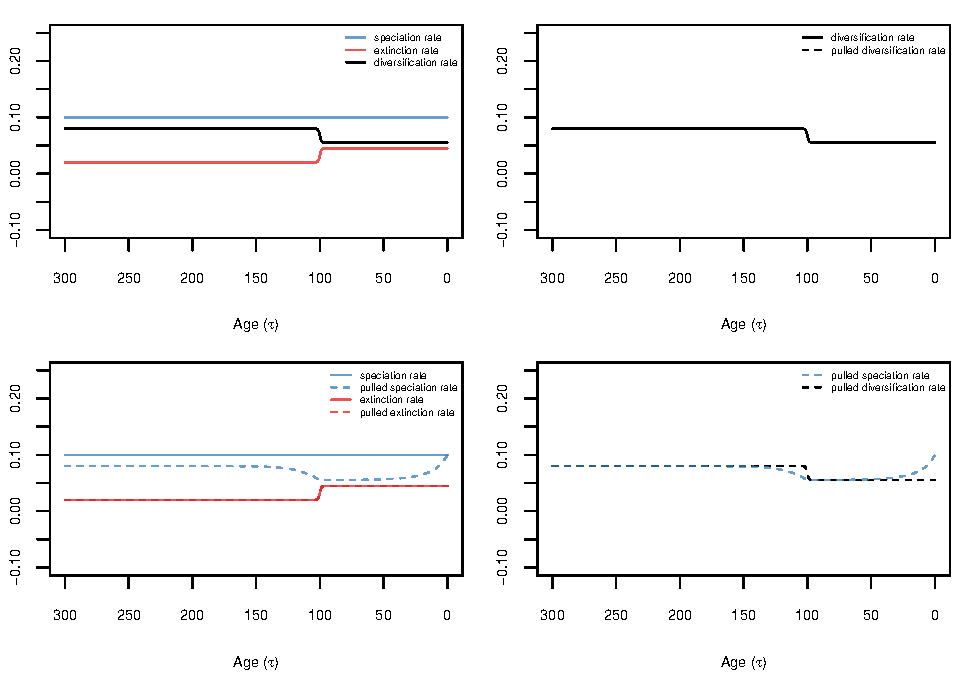
\includegraphics{supplement_files/figure-latex/unnamed-chunk-9-1.pdf}

\pagebreak

\hypertarget{exponential-growth-or-decline-in-speciation-rate}{%
\subsection{Exponential growth or decline in speciation
rate}\label{exponential-growth-or-decline-in-speciation-rate}}

Here we demonstrate a special case where
\(\frac{1}{\lambda} \frac{d\lambda}{d\tau}\) is constant (\(= a\)) so
that \(r_p = r + a\). Variations in \(r_p\) match variations in \(r\)
but the absolute values are different. We present a couple of examples,
first with a gradual exponential increase in speciation rate and a
single gradual change in extinction rate.

\begin{Shaded}
\begin{Highlighting}[]
\NormalTok{tmax }\OtherTok{\textless{}{-}} \DecValTok{300}
\NormalTok{seq\_time }\OtherTok{\textless{}{-}} \FunctionTok{seq}\NormalTok{(}\DecValTok{0}\NormalTok{, tmax, }\FloatTok{0.1}\NormalTok{)}
\NormalTok{spe1 }\OtherTok{\textless{}{-}} \ControlFlowTok{function}\NormalTok{(x) }\FloatTok{0.06} \SpecialCharTok{*} \FunctionTok{exp}\NormalTok{(}\SpecialCharTok{{-}}\FloatTok{0.008} \SpecialCharTok{*}\NormalTok{ x)}
\NormalTok{ext1 }\OtherTok{\textless{}{-}} \ControlFlowTok{function}\NormalTok{(x) }\FunctionTok{smooth\_stepwise}\NormalTok{(}\AttributeTok{r0 =} \FloatTok{0.01}\NormalTok{, }\AttributeTok{r1 =} \FloatTok{0.03}\NormalTok{, }\AttributeTok{Tshift =} \DecValTok{100}\NormalTok{,}
    \AttributeTok{alpha =} \FloatTok{0.05}\NormalTok{, x)}
\FunctionTok{plot\_scenario}\NormalTok{(}\AttributeTok{spe =}\NormalTok{ spe1, }\AttributeTok{ext =}\NormalTok{ ext1, }\AttributeTok{rho =} \DecValTok{1}\NormalTok{, }\AttributeTok{seq\_time =} \FunctionTok{seq}\NormalTok{(}\DecValTok{0}\NormalTok{,}
\NormalTok{    tmax, }\FloatTok{0.1}\NormalTok{))}
\end{Highlighting}
\end{Shaded}

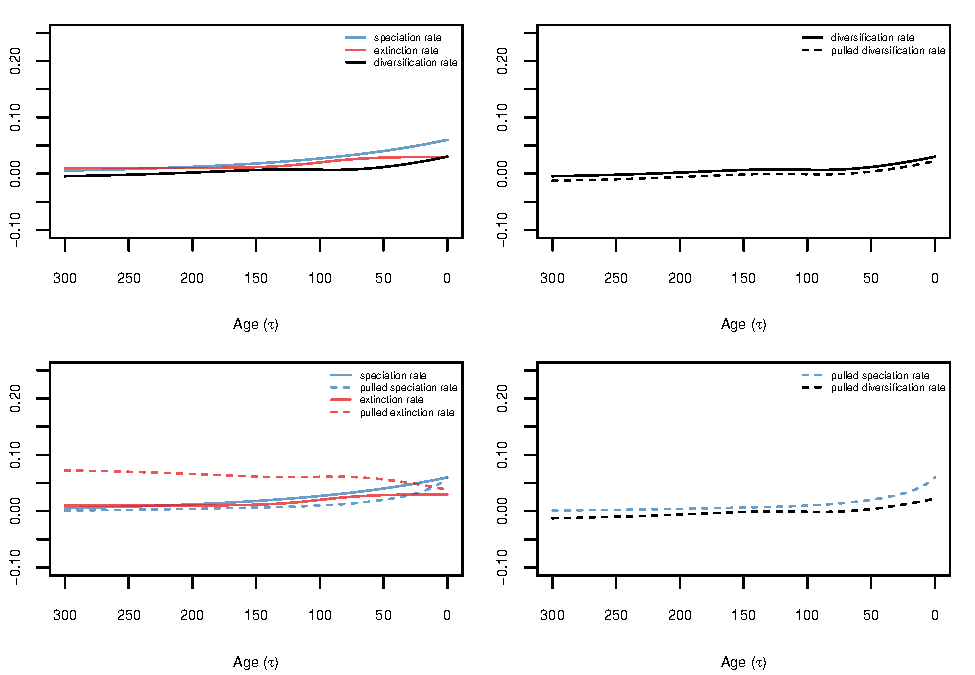
\includegraphics{supplement_files/figure-latex/unnamed-chunk-10-1.pdf}

\pagebreak

A more rapid exponential increase in speciation rate, with an
oscillating extinction rate. Note how the oscillations in \(r_p\) and
\(r\) mirror each other.

\begin{Shaded}
\begin{Highlighting}[]
\NormalTok{tmax }\OtherTok{\textless{}{-}} \DecValTok{300}
\NormalTok{seq\_time }\OtherTok{\textless{}{-}} \FunctionTok{seq}\NormalTok{(}\DecValTok{0}\NormalTok{, tmax, }\FloatTok{0.1}\NormalTok{)}
\NormalTok{spe1 }\OtherTok{\textless{}{-}} \ControlFlowTok{function}\NormalTok{(x) }\FloatTok{0.2} \SpecialCharTok{*} \FunctionTok{exp}\NormalTok{(}\SpecialCharTok{{-}}\FloatTok{0.01} \SpecialCharTok{*}\NormalTok{ x)}
\NormalTok{ext1 }\OtherTok{\textless{}{-}} \ControlFlowTok{function}\NormalTok{(x) }\FloatTok{0.02} \SpecialCharTok{*}\NormalTok{ (}\FloatTok{1.1} \SpecialCharTok{+} \FloatTok{0.5} \SpecialCharTok{*} \FunctionTok{cos}\NormalTok{(}\FloatTok{0.1} \SpecialCharTok{*}\NormalTok{ x))}
\FunctionTok{plot\_scenario}\NormalTok{(}\AttributeTok{spe =}\NormalTok{ spe1, }\AttributeTok{ext =}\NormalTok{ ext1, }\AttributeTok{rho =} \DecValTok{1}\NormalTok{, }\AttributeTok{seq\_time =} \FunctionTok{seq}\NormalTok{(}\DecValTok{0}\NormalTok{,}
\NormalTok{    tmax, }\FloatTok{0.1}\NormalTok{))}
\end{Highlighting}
\end{Shaded}

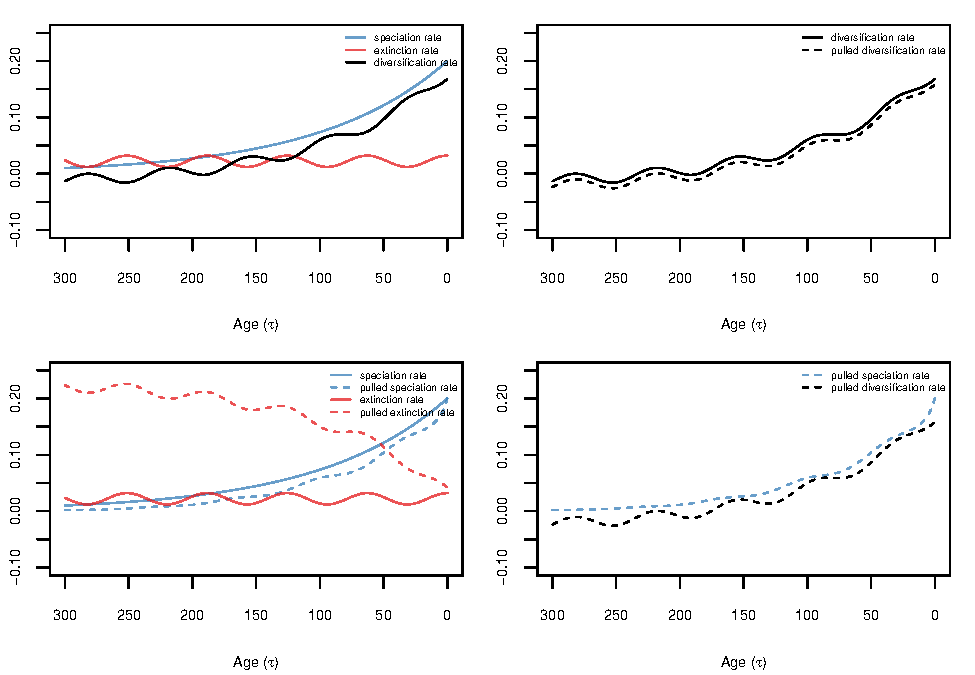
\includegraphics{supplement_files/figure-latex/unnamed-chunk-11-1.pdf}

\pagebreak

\hypertarget{contrasted-scenarios-for-speciation-and-extinction-leading-to-a-similar-scenario-for-diversification}{%
\subsection{Contrasted scenarios for speciation and extinction leading
to a similar scenario for
diversification}\label{contrasted-scenarios-for-speciation-and-extinction-leading-to-a-similar-scenario-for-diversification}}

In their article, LP give an example with flowering plants, fitting two
congruent models in which patterns of speciation and extinction
variation strongly differ - both rates are either increasing or
decreasing through time. However, the resulting pattern in
diversification can be quite similar between the two scenarios, which we
highlight here with two examples with contrasting scenarios. First, a
scenario where both speciation and extinction rates are increasing.

\begin{Shaded}
\begin{Highlighting}[]
\NormalTok{tmax }\OtherTok{\textless{}{-}} \DecValTok{300}
\NormalTok{seq\_time }\OtherTok{\textless{}{-}} \FunctionTok{seq}\NormalTok{(}\DecValTok{0}\NormalTok{, tmax, }\FloatTok{0.1}\NormalTok{)}
\NormalTok{spe1 }\OtherTok{\textless{}{-}} \ControlFlowTok{function}\NormalTok{(x) }\FloatTok{0.05} \SpecialCharTok{+} \FloatTok{2e{-}04} \SpecialCharTok{*}\NormalTok{ x}
\NormalTok{ext1 }\OtherTok{\textless{}{-}} \ControlFlowTok{function}\NormalTok{(x) }\FloatTok{0.02} \SpecialCharTok{+} \FloatTok{1e{-}04} \SpecialCharTok{*}\NormalTok{ x}
\FunctionTok{plot\_scenario}\NormalTok{(}\AttributeTok{spe =}\NormalTok{ spe1, }\AttributeTok{ext =}\NormalTok{ ext1, }\AttributeTok{rho =} \DecValTok{1}\NormalTok{, }\AttributeTok{seq\_time =} \FunctionTok{seq}\NormalTok{(}\DecValTok{0}\NormalTok{,}
\NormalTok{    tmax, }\FloatTok{0.1}\NormalTok{))}
\end{Highlighting}
\end{Shaded}

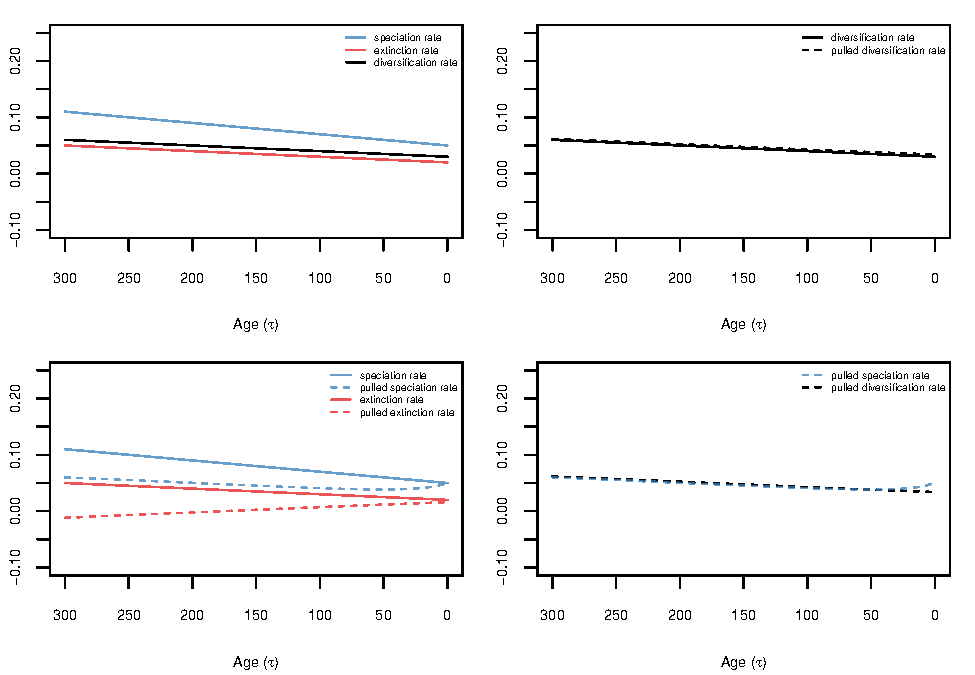
\includegraphics{supplement_files/figure-latex/unnamed-chunk-12-1.pdf}

\pagebreak

Second, a scenario in which both speciation and extinction rate
decreasing. Note how diversification rate remains similar between the
two scenarios.

\begin{Shaded}
\begin{Highlighting}[]
\NormalTok{tmax }\OtherTok{\textless{}{-}} \DecValTok{300}
\NormalTok{seq\_time }\OtherTok{\textless{}{-}} \FunctionTok{seq}\NormalTok{(}\DecValTok{0}\NormalTok{, tmax, }\FloatTok{0.1}\NormalTok{)}
\NormalTok{spe1 }\OtherTok{\textless{}{-}} \ControlFlowTok{function}\NormalTok{(x) }\FloatTok{0.1} \SpecialCharTok{{-}} \FloatTok{1e{-}04} \SpecialCharTok{*}\NormalTok{ x}
\NormalTok{ext1 }\OtherTok{\textless{}{-}} \ControlFlowTok{function}\NormalTok{(x) }\FloatTok{0.07} \SpecialCharTok{{-}} \FloatTok{2e{-}04} \SpecialCharTok{*}\NormalTok{ x}
\FunctionTok{plot\_scenario}\NormalTok{(}\AttributeTok{spe =}\NormalTok{ spe1, }\AttributeTok{ext =}\NormalTok{ ext1, }\AttributeTok{rho =} \DecValTok{1}\NormalTok{, }\AttributeTok{seq\_time =} \FunctionTok{seq}\NormalTok{(}\DecValTok{0}\NormalTok{,}
\NormalTok{    tmax, }\FloatTok{0.1}\NormalTok{))}
\end{Highlighting}
\end{Shaded}

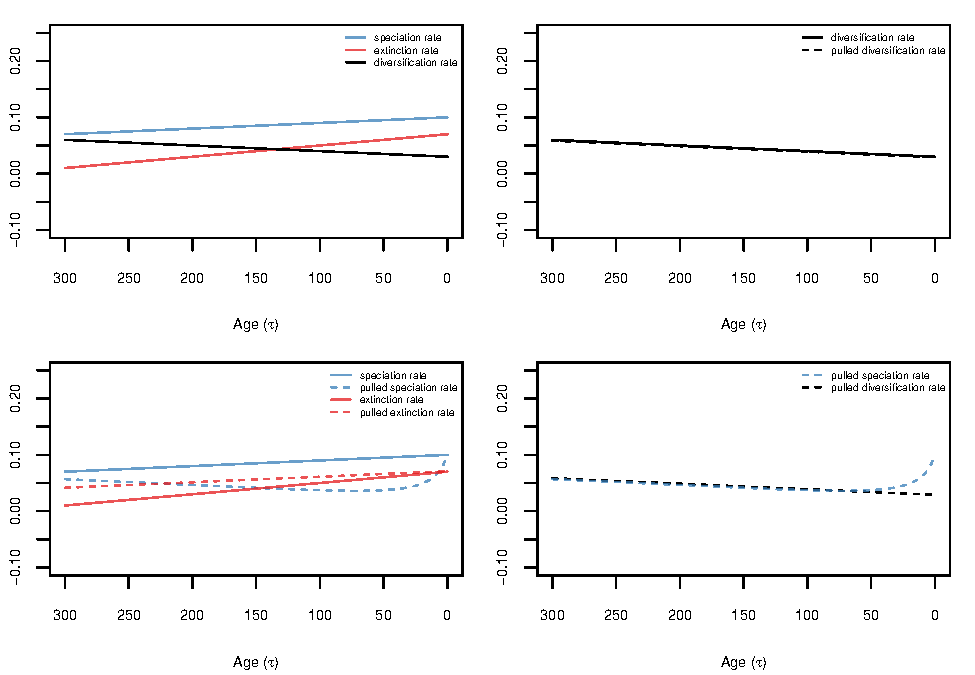
\includegraphics{supplement_files/figure-latex/unnamed-chunk-13-1.pdf}

\pagebreak

\hypertarget{uncorrelated-variations-in-both-rates}{%
\subsection{Uncorrelated variations in both
rates}\label{uncorrelated-variations-in-both-rates}}

In such scenarios, \(r_p\) is usually close to \(r\) except during rapid
shifts in \(\lambda\), which can be detected by comparing the
identifiable rates, \(r_p\) and \(\lambda_p\). Below are a few examples.

\begin{Shaded}
\begin{Highlighting}[]
\NormalTok{tmax }\OtherTok{\textless{}{-}} \DecValTok{300}
\NormalTok{seq\_time }\OtherTok{\textless{}{-}} \FunctionTok{seq}\NormalTok{(}\DecValTok{0}\NormalTok{, tmax, }\FloatTok{0.1}\NormalTok{)}
\NormalTok{spe1 }\OtherTok{\textless{}{-}} \ControlFlowTok{function}\NormalTok{(x) }\FunctionTok{ifelse}\NormalTok{(x }\SpecialCharTok{\textless{}} \DecValTok{150}\NormalTok{, }\FunctionTok{smooth\_stepwise}\NormalTok{(}\AttributeTok{r0 =} \FloatTok{0.1}\NormalTok{,}
    \AttributeTok{r1 =} \FloatTok{0.05}\NormalTok{, }\AttributeTok{Tshift =} \DecValTok{120}\NormalTok{, }\AttributeTok{alpha =} \FloatTok{0.5}\NormalTok{, x), }\FunctionTok{smooth\_stepwise}\NormalTok{(}\AttributeTok{r0 =} \FloatTok{0.04}\NormalTok{,}
    \AttributeTok{r1 =} \FloatTok{0.1}\NormalTok{, }\AttributeTok{Tshift =} \DecValTok{200}\NormalTok{, }\AttributeTok{alpha =} \FloatTok{0.5}\NormalTok{, x))}
\NormalTok{ext1 }\OtherTok{\textless{}{-}} \ControlFlowTok{function}\NormalTok{(x) }\FunctionTok{ifelse}\NormalTok{(x }\SpecialCharTok{\textless{}} \DecValTok{75}\NormalTok{, }\FunctionTok{smooth\_stepwise}\NormalTok{(}\AttributeTok{r0 =} \FloatTok{0.01}\NormalTok{,}
    \AttributeTok{r1 =} \FloatTok{0.04}\NormalTok{, }\AttributeTok{Tshift =} \DecValTok{50}\NormalTok{, }\AttributeTok{alpha =} \FloatTok{0.5}\NormalTok{, x), }\FunctionTok{smooth\_stepwise}\NormalTok{(}\AttributeTok{r0 =} \FloatTok{0.04}\NormalTok{,}
    \AttributeTok{r1 =} \FloatTok{0.01}\NormalTok{, }\AttributeTok{Tshift =} \DecValTok{80}\NormalTok{, }\AttributeTok{alpha =} \FloatTok{0.5}\NormalTok{, x))}
\FunctionTok{plot\_scenario}\NormalTok{(}\AttributeTok{spe =}\NormalTok{ spe1, }\AttributeTok{ext =}\NormalTok{ ext1, }\AttributeTok{rho =} \DecValTok{1}\NormalTok{, }\AttributeTok{seq\_time =} \FunctionTok{seq}\NormalTok{(}\DecValTok{0}\NormalTok{,}
\NormalTok{    tmax, }\FloatTok{0.1}\NormalTok{))}
\end{Highlighting}
\end{Shaded}

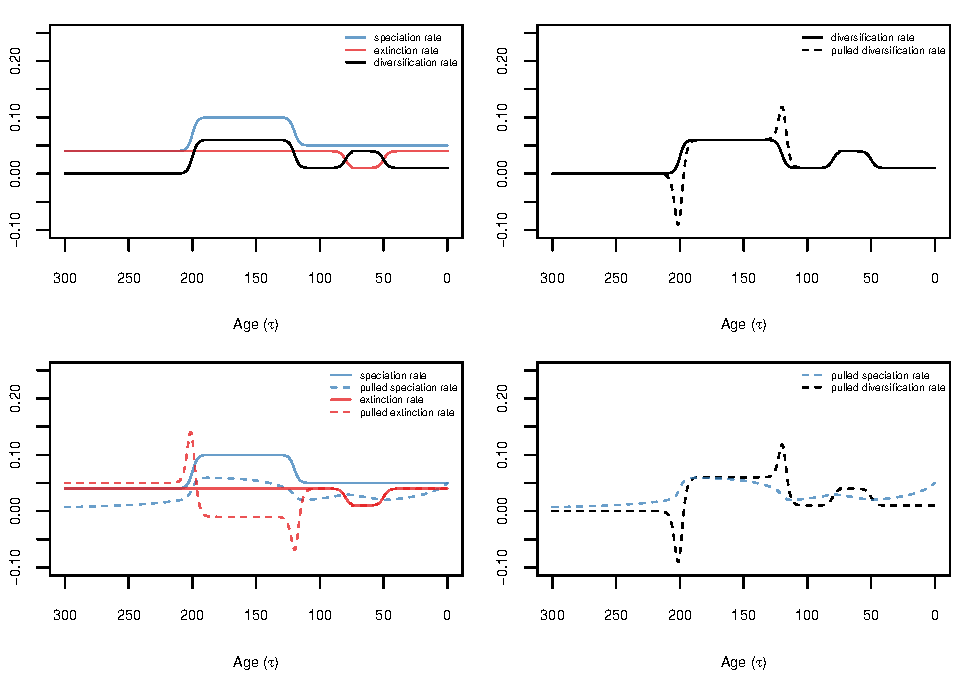
\includegraphics{supplement_files/figure-latex/unnamed-chunk-14-1.pdf}

\pagebreak

\begin{Shaded}
\begin{Highlighting}[]
\NormalTok{tmax }\OtherTok{\textless{}{-}} \DecValTok{300}
\NormalTok{seq\_time }\OtherTok{\textless{}{-}} \FunctionTok{seq}\NormalTok{(}\DecValTok{0}\NormalTok{, tmax, }\FloatTok{0.1}\NormalTok{)}
\NormalTok{spe1 }\OtherTok{\textless{}{-}} \ControlFlowTok{function}\NormalTok{(x) }\FloatTok{0.05} \SpecialCharTok{*}\NormalTok{ (}\DecValTok{1} \SpecialCharTok{+} \FunctionTok{exp}\NormalTok{(}\SpecialCharTok{{-}}\NormalTok{(x }\SpecialCharTok{{-}} \DecValTok{100}\NormalTok{)}\SpecialCharTok{\^{}}\DecValTok{2}\SpecialCharTok{/}\DecValTok{100}\NormalTok{) }\SpecialCharTok{{-}} \FloatTok{0.5} \SpecialCharTok{*}
    \FunctionTok{exp}\NormalTok{(}\SpecialCharTok{{-}}\NormalTok{(x }\SpecialCharTok{{-}} \DecValTok{200}\NormalTok{)}\SpecialCharTok{\^{}}\DecValTok{2}\SpecialCharTok{/}\DecValTok{200}\NormalTok{))}
\NormalTok{ext1 }\OtherTok{\textless{}{-}} \ControlFlowTok{function}\NormalTok{(x) }\FloatTok{0.02} \SpecialCharTok{*}\NormalTok{ (}\DecValTok{1} \SpecialCharTok{{-}} \FloatTok{0.5} \SpecialCharTok{*} \FunctionTok{exp}\NormalTok{(}\SpecialCharTok{{-}}\NormalTok{(x }\SpecialCharTok{{-}} \DecValTok{50}\NormalTok{)}\SpecialCharTok{\^{}}\DecValTok{2}\SpecialCharTok{/}\DecValTok{100}\NormalTok{) }\SpecialCharTok{+}
    \FunctionTok{exp}\NormalTok{(}\SpecialCharTok{{-}}\NormalTok{(x }\SpecialCharTok{{-}} \DecValTok{180}\NormalTok{)}\SpecialCharTok{\^{}}\DecValTok{2}\SpecialCharTok{/}\DecValTok{300}\NormalTok{))}
\FunctionTok{plot\_scenario}\NormalTok{(}\AttributeTok{spe =}\NormalTok{ spe1, }\AttributeTok{ext =}\NormalTok{ ext1, }\AttributeTok{rho =} \DecValTok{1}\NormalTok{, }\AttributeTok{seq\_time =} \FunctionTok{seq}\NormalTok{(}\DecValTok{0}\NormalTok{,}
\NormalTok{    tmax, }\FloatTok{0.1}\NormalTok{))}
\end{Highlighting}
\end{Shaded}

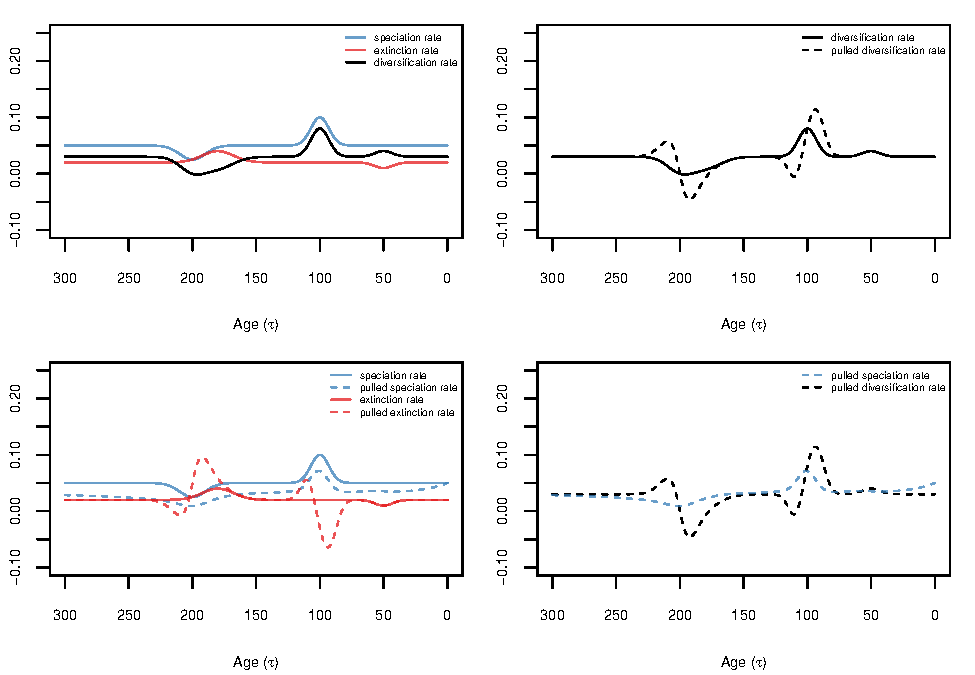
\includegraphics{supplement_files/figure-latex/unnamed-chunk-15-1.pdf}

\pagebreak

\begin{Shaded}
\begin{Highlighting}[]
\NormalTok{tmax }\OtherTok{\textless{}{-}} \DecValTok{300}
\NormalTok{seq\_time }\OtherTok{\textless{}{-}} \FunctionTok{seq}\NormalTok{(}\DecValTok{0}\NormalTok{, tmax, }\FloatTok{0.1}\NormalTok{)}
\NormalTok{spe1 }\OtherTok{\textless{}{-}} \ControlFlowTok{function}\NormalTok{(x) }\FloatTok{0.05} \SpecialCharTok{*}\NormalTok{ (}\DecValTok{1} \SpecialCharTok{+} \FloatTok{0.2} \SpecialCharTok{*} \FunctionTok{cos}\NormalTok{(}\FloatTok{0.05} \SpecialCharTok{*}\NormalTok{ x))}
\NormalTok{ext1 }\OtherTok{\textless{}{-}} \ControlFlowTok{function}\NormalTok{(x) }\FloatTok{0.02} \SpecialCharTok{*}\NormalTok{ (}\DecValTok{1} \SpecialCharTok{{-}} \FloatTok{0.5} \SpecialCharTok{*} \FunctionTok{exp}\NormalTok{(}\SpecialCharTok{{-}}\NormalTok{(x }\SpecialCharTok{{-}} \DecValTok{50}\NormalTok{)}\SpecialCharTok{\^{}}\DecValTok{2}\SpecialCharTok{/}\DecValTok{100}\NormalTok{) }\SpecialCharTok{+}
    \FunctionTok{exp}\NormalTok{(}\SpecialCharTok{{-}}\NormalTok{(x }\SpecialCharTok{{-}} \DecValTok{180}\NormalTok{)}\SpecialCharTok{\^{}}\DecValTok{2}\SpecialCharTok{/}\DecValTok{300}\NormalTok{))}
\FunctionTok{plot\_scenario}\NormalTok{(}\AttributeTok{spe =}\NormalTok{ spe1, }\AttributeTok{ext =}\NormalTok{ ext1, }\AttributeTok{rho =} \DecValTok{1}\NormalTok{, }\AttributeTok{seq\_time =} \FunctionTok{seq}\NormalTok{(}\DecValTok{0}\NormalTok{,}
\NormalTok{    tmax, }\FloatTok{0.1}\NormalTok{))}
\end{Highlighting}
\end{Shaded}

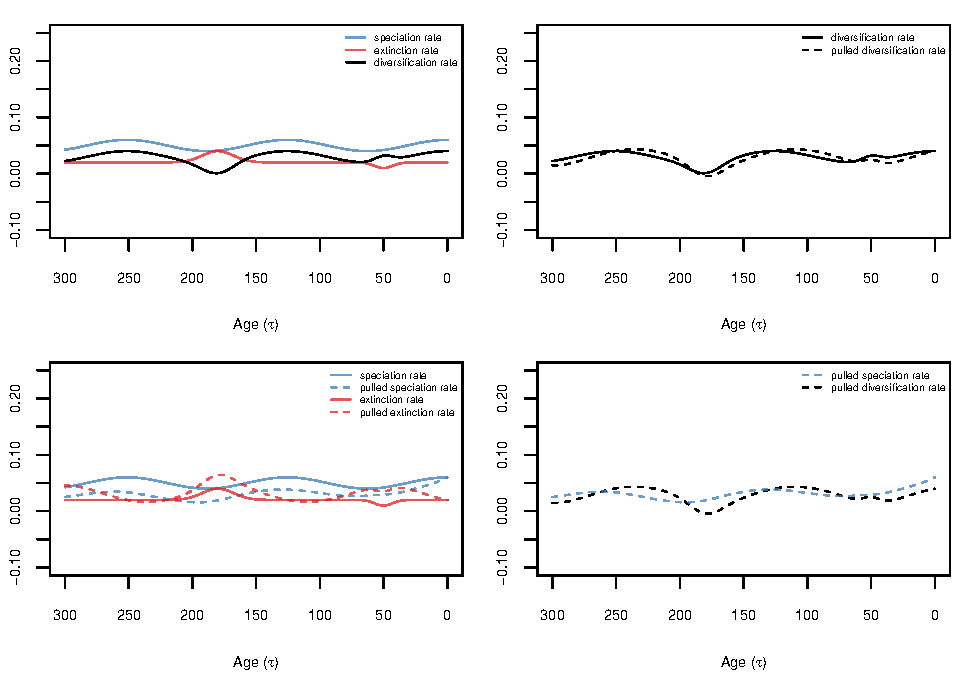
\includegraphics{supplement_files/figure-latex/unnamed-chunk-16-1.pdf}

\pagebreak

\hypertarget{the-worst-case-scenario-parallel-variation-in-speciation-and-extinction-rates}{%
\subsection{The worst case scenario : parallel variation in speciation
and extinction
rates}\label{the-worst-case-scenario-parallel-variation-in-speciation-and-extinction-rates}}

According to the definition of \(r_p\), the worst case is expected when
\(\lambda\) varies but \(r\) is constant, that is when
\(\mu = \lambda - b\) where \(b\) is a constant. If so, \(r\) is
constant whereas \(r_p\) varies so that \(r_p\) can be a very poor
predictor of \(r\). We start with a gradual change in rates so \(r_p\)
only slightly departs from \(r\).

\begin{Shaded}
\begin{Highlighting}[]
\NormalTok{tmax }\OtherTok{\textless{}{-}} \DecValTok{300}
\NormalTok{seq\_time }\OtherTok{\textless{}{-}} \FunctionTok{seq}\NormalTok{(}\DecValTok{0}\NormalTok{, tmax, }\FloatTok{0.1}\NormalTok{)}
\NormalTok{spe1 }\OtherTok{\textless{}{-}} \ControlFlowTok{function}\NormalTok{(x) }\FloatTok{0.05} \SpecialCharTok{+} \FloatTok{0.05} \SpecialCharTok{*} \FunctionTok{exp}\NormalTok{(}\SpecialCharTok{{-}}\FloatTok{0.02} \SpecialCharTok{*}\NormalTok{ x)}
\NormalTok{ext1 }\OtherTok{\textless{}{-}} \ControlFlowTok{function}\NormalTok{(x) }\FloatTok{0.045} \SpecialCharTok{+} \FloatTok{0.05} \SpecialCharTok{*} \FunctionTok{exp}\NormalTok{(}\SpecialCharTok{{-}}\FloatTok{0.02} \SpecialCharTok{*}\NormalTok{ x)}
\FunctionTok{plot\_scenario}\NormalTok{(}\AttributeTok{spe =}\NormalTok{ spe1, }\AttributeTok{ext =}\NormalTok{ ext1, }\AttributeTok{rho =} \DecValTok{1}\NormalTok{, }\AttributeTok{seq\_time =} \FunctionTok{seq}\NormalTok{(}\DecValTok{0}\NormalTok{,}
\NormalTok{    tmax, }\FloatTok{0.1}\NormalTok{))}
\end{Highlighting}
\end{Shaded}

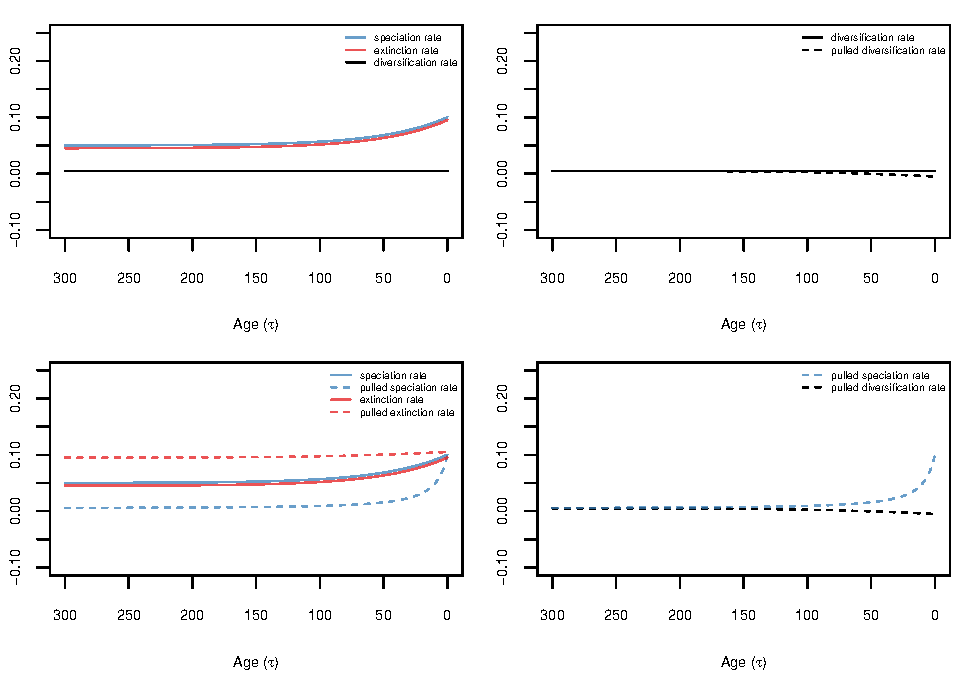
\includegraphics{supplement_files/figure-latex/unnamed-chunk-17-1.pdf}

\pagebreak

As we increased the complexity of the parallel changes in rates, \(r_p\)
and \(r\) begin to differ more.

\begin{Shaded}
\begin{Highlighting}[]
\NormalTok{tmax }\OtherTok{\textless{}{-}} \DecValTok{300}
\NormalTok{seq\_time }\OtherTok{\textless{}{-}} \FunctionTok{seq}\NormalTok{(}\DecValTok{0}\NormalTok{, tmax, }\FloatTok{0.1}\NormalTok{)}
\NormalTok{spe1 }\OtherTok{\textless{}{-}} \ControlFlowTok{function}\NormalTok{(x) }\FloatTok{0.05} \SpecialCharTok{+} \FloatTok{0.05} \SpecialCharTok{*} \FunctionTok{exp}\NormalTok{(}\SpecialCharTok{{-}}\NormalTok{(x }\SpecialCharTok{{-}} \DecValTok{50}\NormalTok{)}\SpecialCharTok{\^{}}\DecValTok{2}\SpecialCharTok{/}\DecValTok{500}\NormalTok{) }\SpecialCharTok{+} \FloatTok{0.1} \SpecialCharTok{*}
    \FunctionTok{exp}\NormalTok{(}\SpecialCharTok{{-}}\NormalTok{(x }\SpecialCharTok{{-}} \DecValTok{200}\NormalTok{)}\SpecialCharTok{\^{}}\DecValTok{2}\SpecialCharTok{/}\DecValTok{10000}\NormalTok{)}
\NormalTok{ext1 }\OtherTok{\textless{}{-}} \ControlFlowTok{function}\NormalTok{(x) }\FloatTok{0.02} \SpecialCharTok{+} \FloatTok{0.05} \SpecialCharTok{*} \FunctionTok{exp}\NormalTok{(}\SpecialCharTok{{-}}\NormalTok{(x }\SpecialCharTok{{-}} \DecValTok{50}\NormalTok{)}\SpecialCharTok{\^{}}\DecValTok{2}\SpecialCharTok{/}\DecValTok{500}\NormalTok{) }\SpecialCharTok{+} \FloatTok{0.1} \SpecialCharTok{*}
    \FunctionTok{exp}\NormalTok{(}\SpecialCharTok{{-}}\NormalTok{(x }\SpecialCharTok{{-}} \DecValTok{200}\NormalTok{)}\SpecialCharTok{\^{}}\DecValTok{2}\SpecialCharTok{/}\DecValTok{10000}\NormalTok{)}
\FunctionTok{plot\_scenario}\NormalTok{(}\AttributeTok{spe =}\NormalTok{ spe1, }\AttributeTok{ext =}\NormalTok{ ext1, }\AttributeTok{rho =} \DecValTok{1}\NormalTok{, }\AttributeTok{seq\_time =} \FunctionTok{seq}\NormalTok{(}\DecValTok{0}\NormalTok{,}
\NormalTok{    tmax, }\FloatTok{0.1}\NormalTok{))}
\end{Highlighting}
\end{Shaded}

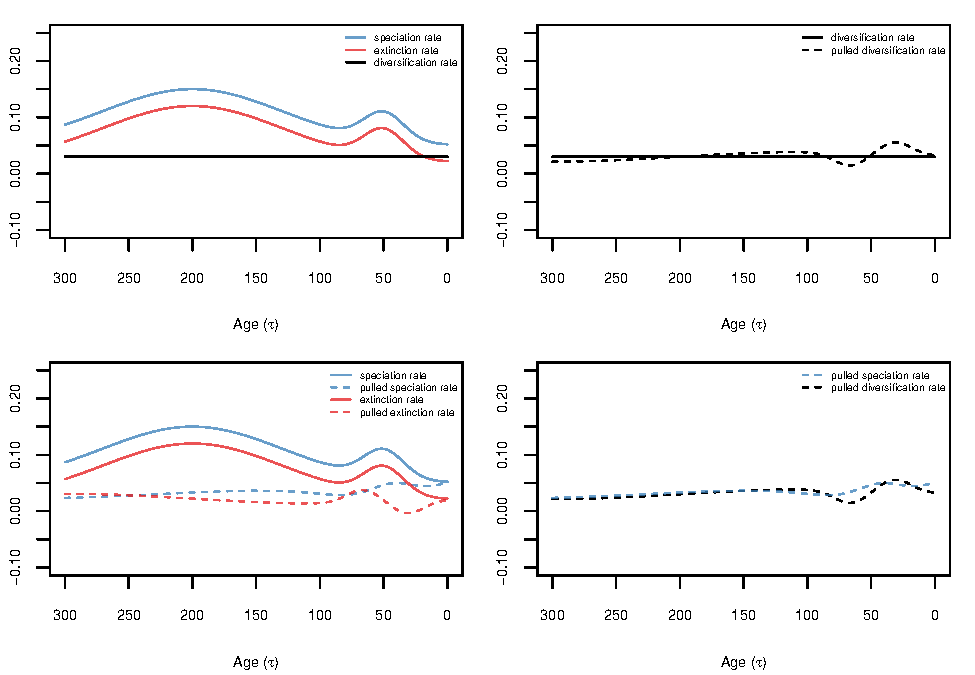
\includegraphics{supplement_files/figure-latex/unnamed-chunk-18-1.pdf}

\pagebreak

To illustrate an extreme case, here are rapid and parallel variations in
speciation and extinction rate, resulting in an \(r_p\) that varies with
equal rapidity but bears no resemblence to \(r\), which remains
constant. Also note how \(r_p\) and \(\lambda_p\) are very different,
which we suggest is a good indicator that \(r_p\) is not a good
representation of \(r\).

\begin{Shaded}
\begin{Highlighting}[]
\NormalTok{tmax }\OtherTok{\textless{}{-}} \DecValTok{300}
\NormalTok{seq\_time }\OtherTok{\textless{}{-}} \FunctionTok{seq}\NormalTok{(}\DecValTok{0}\NormalTok{, tmax, }\FloatTok{0.1}\NormalTok{)}
\NormalTok{spe1 }\OtherTok{\textless{}{-}} \ControlFlowTok{function}\NormalTok{(x) }\FloatTok{0.05} \SpecialCharTok{+} \FloatTok{0.015} \SpecialCharTok{*} \FunctionTok{cos}\NormalTok{(}\FloatTok{0.25} \SpecialCharTok{*}\NormalTok{ x)}
\NormalTok{ext1 }\OtherTok{\textless{}{-}} \ControlFlowTok{function}\NormalTok{(x) }\FloatTok{0.02} \SpecialCharTok{+} \FloatTok{0.015} \SpecialCharTok{*} \FunctionTok{cos}\NormalTok{(}\FloatTok{0.25} \SpecialCharTok{*}\NormalTok{ x)}
\FunctionTok{plot\_scenario}\NormalTok{(}\AttributeTok{spe =}\NormalTok{ spe1, }\AttributeTok{ext =}\NormalTok{ ext1, }\AttributeTok{rho =} \DecValTok{1}\NormalTok{, }\AttributeTok{seq\_time =} \FunctionTok{seq}\NormalTok{(}\DecValTok{0}\NormalTok{,}
\NormalTok{    tmax, }\FloatTok{0.1}\NormalTok{))}
\end{Highlighting}
\end{Shaded}

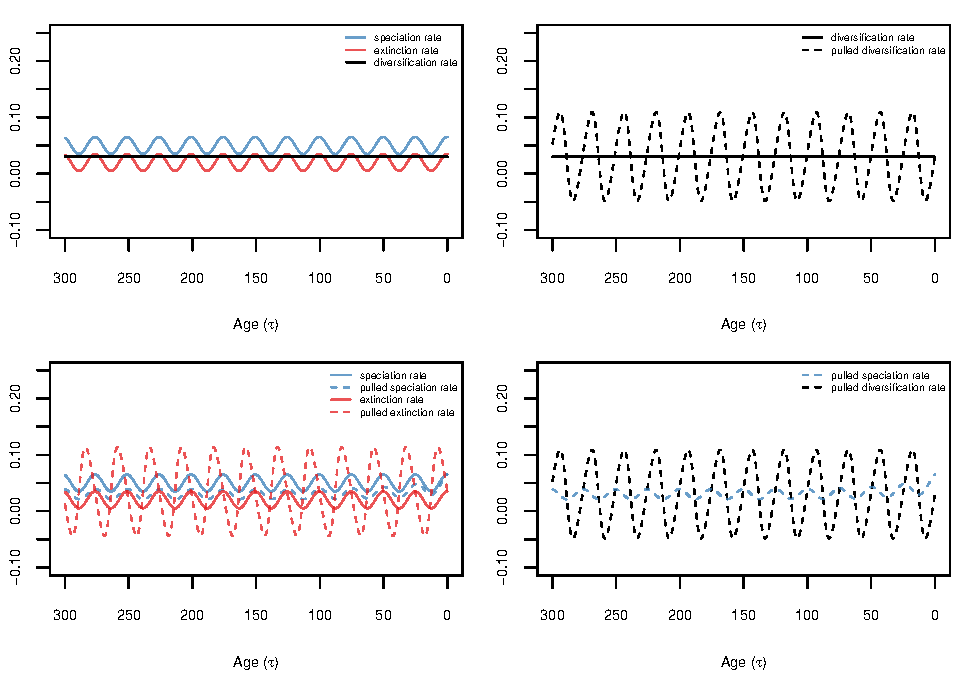
\includegraphics{supplement_files/figure-latex/unnamed-chunk-19-1.pdf}

\pagebreak

\hypertarget{how-sensitive-is-r_p-to-variations-in-lambda-and-mu}{%
\subsection{\texorpdfstring{How sensitive is \(r_p\) to variations in
\(\lambda\) and
\(\mu\)?}{How sensitive is r\_p to variations in \textbackslash lambda and \textbackslash mu?}}\label{how-sensitive-is-r_p-to-variations-in-lambda-and-mu}}

Sinusoidal functions are useful to assess the sensitivity of these
results. Discrepancies are stronger when \(r\) is constant, so how
variable does \(r\) have to be for \(r_p\) to be a good approximation of
\(r\)? The following graphs explore how slight differences in the
amplitude, period and phase of the variations in speciation and
extinction rate alter the results presented above, where variations are
parallel. If a slight change is introduced then \(r_p\) and \(r\) become
almost immediately similar. Variation in the period is particularly
effective. Quantitative differences still persist when amplitude and
phase are changed, but the qualitative behavior becomes more similar
i.e.~the shape of the curves is similar, even if they are delayed for
\(r_p\).

\pagebreak

Here we introduce a slight difference in the amplitude, the degree to
which rates vary, by increasing amplitude for speciation rate. The top
left panel shows parallel rates and amplitude is gradually increased in
the other panels.

\begin{Shaded}
\begin{Highlighting}[]
\NormalTok{spe }\OtherTok{\textless{}{-}} \FunctionTok{list}\NormalTok{()}
\NormalTok{ext }\OtherTok{\textless{}{-}} \FunctionTok{list}\NormalTok{()}

\NormalTok{spe[[}\DecValTok{1}\NormalTok{]] }\OtherTok{\textless{}{-}} \ControlFlowTok{function}\NormalTok{(x) }\FloatTok{0.05} \SpecialCharTok{+} \FloatTok{0.01} \SpecialCharTok{*} \FunctionTok{cos}\NormalTok{(}\FloatTok{0.05} \SpecialCharTok{*}\NormalTok{ x)}
\NormalTok{ext[[}\DecValTok{1}\NormalTok{]] }\OtherTok{\textless{}{-}} \ControlFlowTok{function}\NormalTok{(x) }\FloatTok{0.02} \SpecialCharTok{+} \FloatTok{0.01} \SpecialCharTok{*} \FunctionTok{cos}\NormalTok{(}\FloatTok{0.05} \SpecialCharTok{*}\NormalTok{ x)}

\NormalTok{spe[[}\DecValTok{2}\NormalTok{]] }\OtherTok{\textless{}{-}} \ControlFlowTok{function}\NormalTok{(x) }\FloatTok{0.05} \SpecialCharTok{+} \FloatTok{0.015} \SpecialCharTok{*} \FunctionTok{cos}\NormalTok{(}\FloatTok{0.05} \SpecialCharTok{*}\NormalTok{ x)}
\NormalTok{ext[[}\DecValTok{2}\NormalTok{]] }\OtherTok{\textless{}{-}} \ControlFlowTok{function}\NormalTok{(x) }\FloatTok{0.02} \SpecialCharTok{+} \FloatTok{0.01} \SpecialCharTok{*} \FunctionTok{cos}\NormalTok{(}\FloatTok{0.05} \SpecialCharTok{*}\NormalTok{ x)}

\NormalTok{spe[[}\DecValTok{3}\NormalTok{]] }\OtherTok{\textless{}{-}} \ControlFlowTok{function}\NormalTok{(x) }\FloatTok{0.05} \SpecialCharTok{+} \FloatTok{0.02} \SpecialCharTok{*} \FunctionTok{cos}\NormalTok{(}\FloatTok{0.05} \SpecialCharTok{*}\NormalTok{ x)}
\NormalTok{ext[[}\DecValTok{3}\NormalTok{]] }\OtherTok{\textless{}{-}} \ControlFlowTok{function}\NormalTok{(x) }\FloatTok{0.02} \SpecialCharTok{+} \FloatTok{0.01} \SpecialCharTok{*} \FunctionTok{cos}\NormalTok{(}\FloatTok{0.05} \SpecialCharTok{*}\NormalTok{ x)}

\NormalTok{spe[[}\DecValTok{4}\NormalTok{]] }\OtherTok{\textless{}{-}} \ControlFlowTok{function}\NormalTok{(x) }\FloatTok{0.05} \SpecialCharTok{+} \FloatTok{0.025} \SpecialCharTok{*} \FunctionTok{cos}\NormalTok{(}\FloatTok{0.05} \SpecialCharTok{*}\NormalTok{ x)}
\NormalTok{ext[[}\DecValTok{4}\NormalTok{]] }\OtherTok{\textless{}{-}} \ControlFlowTok{function}\NormalTok{(x) }\FloatTok{0.02} \SpecialCharTok{+} \FloatTok{0.01} \SpecialCharTok{*} \FunctionTok{cos}\NormalTok{(}\FloatTok{0.05} \SpecialCharTok{*}\NormalTok{ x)}
\end{Highlighting}
\end{Shaded}

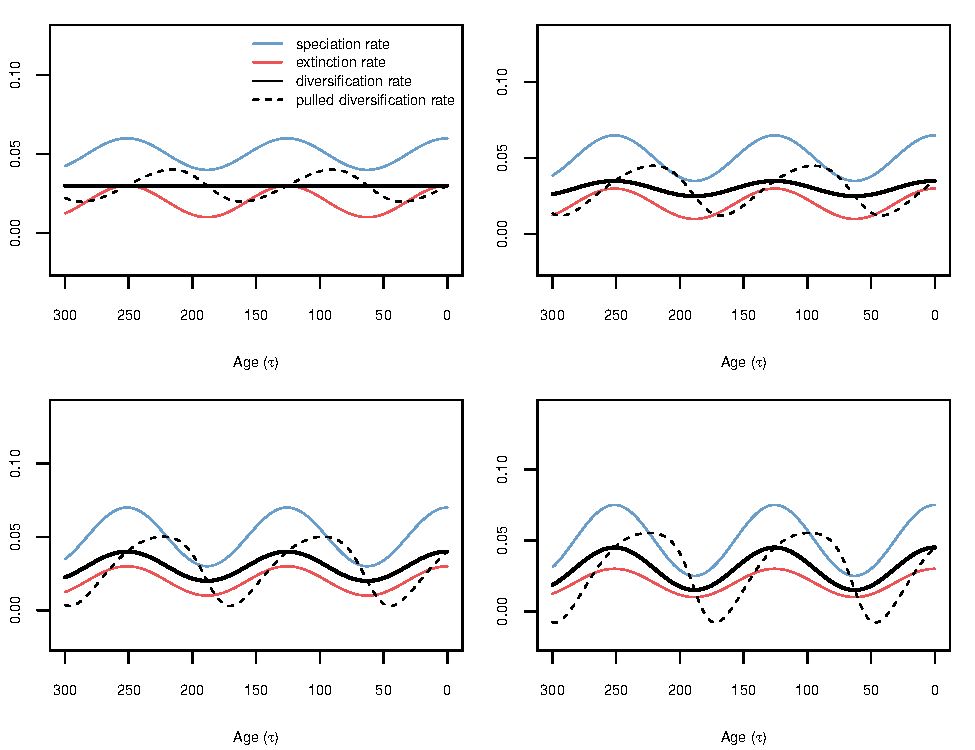
\includegraphics{supplement_files/figure-latex/unnamed-chunk-21-1.pdf}

\pagebreak

Here we show the effect of a slight difference in the period, the rate
at which rates vary, by making speciation rate vary faster than
extinction rate. The top left panel shows parallel rates and period is
gradually increased in the other panels.

\begin{Shaded}
\begin{Highlighting}[]
\NormalTok{tmax }\OtherTok{\textless{}{-}} \DecValTok{300}
\NormalTok{seq\_time }\OtherTok{\textless{}{-}} \FunctionTok{seq}\NormalTok{(}\DecValTok{0}\NormalTok{, tmax, }\FloatTok{0.1}\NormalTok{)}

\NormalTok{spe }\OtherTok{\textless{}{-}} \FunctionTok{list}\NormalTok{()}
\NormalTok{ext }\OtherTok{\textless{}{-}} \FunctionTok{list}\NormalTok{()}

\NormalTok{spe[[}\DecValTok{1}\NormalTok{]] }\OtherTok{\textless{}{-}} \ControlFlowTok{function}\NormalTok{(x) }\FloatTok{0.05} \SpecialCharTok{+} \FloatTok{0.01} \SpecialCharTok{*} \FunctionTok{cos}\NormalTok{(}\FloatTok{0.05} \SpecialCharTok{*}\NormalTok{ x)}
\NormalTok{ext[[}\DecValTok{1}\NormalTok{]] }\OtherTok{\textless{}{-}} \ControlFlowTok{function}\NormalTok{(x) }\FloatTok{0.02} \SpecialCharTok{+} \FloatTok{0.01} \SpecialCharTok{*} \FunctionTok{cos}\NormalTok{(}\FloatTok{0.05} \SpecialCharTok{*}\NormalTok{ x)}

\NormalTok{spe[[}\DecValTok{2}\NormalTok{]] }\OtherTok{\textless{}{-}} \ControlFlowTok{function}\NormalTok{(x) }\FloatTok{0.05} \SpecialCharTok{+} \FloatTok{0.01} \SpecialCharTok{*} \FunctionTok{cos}\NormalTok{(}\FloatTok{0.055} \SpecialCharTok{*}\NormalTok{ x)}
\NormalTok{ext[[}\DecValTok{2}\NormalTok{]] }\OtherTok{\textless{}{-}} \ControlFlowTok{function}\NormalTok{(x) }\FloatTok{0.02} \SpecialCharTok{+} \FloatTok{0.01} \SpecialCharTok{*} \FunctionTok{cos}\NormalTok{(}\FloatTok{0.05} \SpecialCharTok{*}\NormalTok{ x)}

\NormalTok{spe[[}\DecValTok{3}\NormalTok{]] }\OtherTok{\textless{}{-}} \ControlFlowTok{function}\NormalTok{(x) }\FloatTok{0.05} \SpecialCharTok{+} \FloatTok{0.01} \SpecialCharTok{*} \FunctionTok{cos}\NormalTok{(}\FloatTok{0.06} \SpecialCharTok{*}\NormalTok{ x)}
\NormalTok{ext[[}\DecValTok{3}\NormalTok{]] }\OtherTok{\textless{}{-}} \ControlFlowTok{function}\NormalTok{(x) }\FloatTok{0.02} \SpecialCharTok{+} \FloatTok{0.01} \SpecialCharTok{*} \FunctionTok{cos}\NormalTok{(}\FloatTok{0.05} \SpecialCharTok{*}\NormalTok{ x)}

\NormalTok{spe[[}\DecValTok{4}\NormalTok{]] }\OtherTok{\textless{}{-}} \ControlFlowTok{function}\NormalTok{(x) }\FloatTok{0.05} \SpecialCharTok{+} \FloatTok{0.01} \SpecialCharTok{*} \FunctionTok{cos}\NormalTok{(}\FloatTok{0.065} \SpecialCharTok{*}\NormalTok{ x)}
\NormalTok{ext[[}\DecValTok{4}\NormalTok{]] }\OtherTok{\textless{}{-}} \ControlFlowTok{function}\NormalTok{(x) }\FloatTok{0.02} \SpecialCharTok{+} \FloatTok{0.01} \SpecialCharTok{*} \FunctionTok{cos}\NormalTok{(}\FloatTok{0.05} \SpecialCharTok{*}\NormalTok{ x)}
\end{Highlighting}
\end{Shaded}

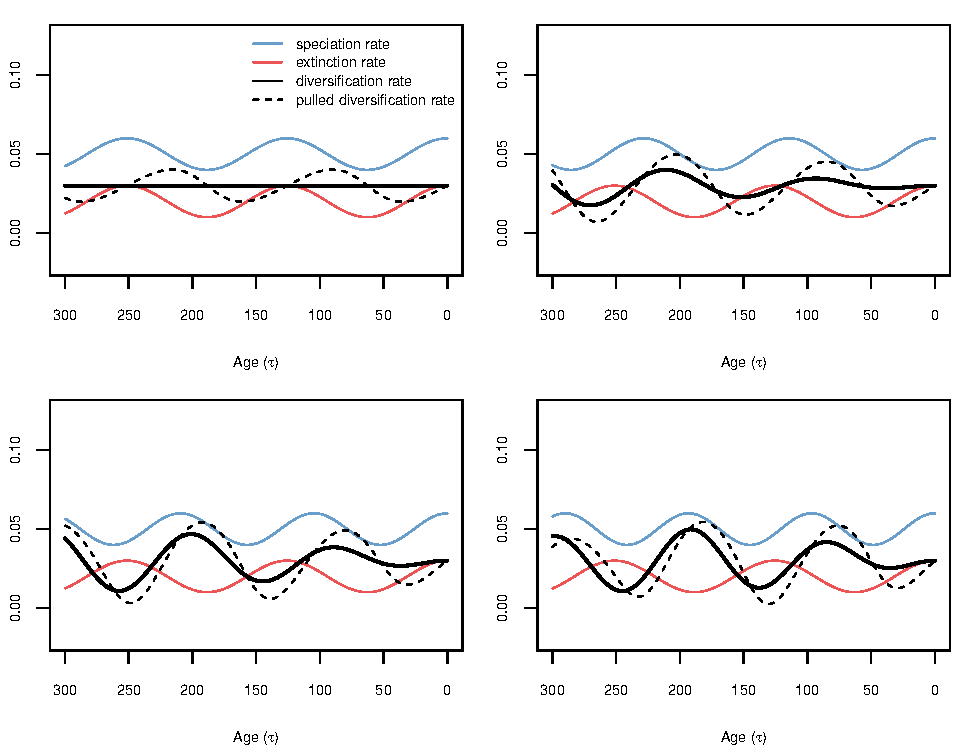
\includegraphics{supplement_files/figure-latex/unnamed-chunk-23-1.pdf}

\pagebreak

Finally we introduce a slight delay in the phase, the timing of the rate
variation, by shifting the curve for speciation rate to the right. The
top left panel shows parallel rates and phadse is gradually shifted in
the other panels.

\begin{Shaded}
\begin{Highlighting}[]
\NormalTok{tmax }\OtherTok{\textless{}{-}} \DecValTok{300}
\NormalTok{seq\_time }\OtherTok{\textless{}{-}} \FunctionTok{seq}\NormalTok{(}\DecValTok{0}\NormalTok{, tmax, }\FloatTok{0.1}\NormalTok{)}

\NormalTok{spe }\OtherTok{\textless{}{-}} \FunctionTok{list}\NormalTok{()}
\NormalTok{ext }\OtherTok{\textless{}{-}} \FunctionTok{list}\NormalTok{()}

\NormalTok{spe[[}\DecValTok{1}\NormalTok{]] }\OtherTok{\textless{}{-}} \ControlFlowTok{function}\NormalTok{(x) }\FloatTok{0.05} \SpecialCharTok{+} \FloatTok{0.01} \SpecialCharTok{*} \FunctionTok{cos}\NormalTok{(}\FloatTok{0.05} \SpecialCharTok{*}\NormalTok{ x)}
\NormalTok{ext[[}\DecValTok{1}\NormalTok{]] }\OtherTok{\textless{}{-}} \ControlFlowTok{function}\NormalTok{(x) }\FloatTok{0.02} \SpecialCharTok{+} \FloatTok{0.01} \SpecialCharTok{*} \FunctionTok{cos}\NormalTok{(}\FloatTok{0.05} \SpecialCharTok{*}\NormalTok{ x)}

\NormalTok{spe[[}\DecValTok{2}\NormalTok{]] }\OtherTok{\textless{}{-}} \ControlFlowTok{function}\NormalTok{(x) }\FloatTok{0.05} \SpecialCharTok{+} \FloatTok{0.01} \SpecialCharTok{*} \FunctionTok{cos}\NormalTok{(}\FloatTok{0.05} \SpecialCharTok{*}\NormalTok{ (x }\SpecialCharTok{{-}} \DecValTok{10}\NormalTok{))}
\NormalTok{ext[[}\DecValTok{2}\NormalTok{]] }\OtherTok{\textless{}{-}} \ControlFlowTok{function}\NormalTok{(x) }\FloatTok{0.02} \SpecialCharTok{+} \FloatTok{0.01} \SpecialCharTok{*} \FunctionTok{cos}\NormalTok{(}\FloatTok{0.05} \SpecialCharTok{*}\NormalTok{ x)}

\NormalTok{spe[[}\DecValTok{3}\NormalTok{]] }\OtherTok{\textless{}{-}} \ControlFlowTok{function}\NormalTok{(x) }\FloatTok{0.05} \SpecialCharTok{+} \FloatTok{0.01} \SpecialCharTok{*} \FunctionTok{cos}\NormalTok{(}\FloatTok{0.05} \SpecialCharTok{*}\NormalTok{ (x }\SpecialCharTok{{-}} \DecValTok{20}\NormalTok{))}
\NormalTok{ext[[}\DecValTok{3}\NormalTok{]] }\OtherTok{\textless{}{-}} \ControlFlowTok{function}\NormalTok{(x) }\FloatTok{0.02} \SpecialCharTok{+} \FloatTok{0.01} \SpecialCharTok{*} \FunctionTok{cos}\NormalTok{(}\FloatTok{0.05} \SpecialCharTok{*}\NormalTok{ x)}

\NormalTok{spe[[}\DecValTok{4}\NormalTok{]] }\OtherTok{\textless{}{-}} \ControlFlowTok{function}\NormalTok{(x) }\FloatTok{0.05} \SpecialCharTok{+} \FloatTok{0.01} \SpecialCharTok{*} \FunctionTok{cos}\NormalTok{(}\FloatTok{0.05} \SpecialCharTok{*}\NormalTok{ (x }\SpecialCharTok{{-}} \DecValTok{30}\NormalTok{))}
\NormalTok{ext[[}\DecValTok{4}\NormalTok{]] }\OtherTok{\textless{}{-}} \ControlFlowTok{function}\NormalTok{(x) }\FloatTok{0.02} \SpecialCharTok{+} \FloatTok{0.01} \SpecialCharTok{*} \FunctionTok{cos}\NormalTok{(}\FloatTok{0.05} \SpecialCharTok{*}\NormalTok{ x)}
\end{Highlighting}
\end{Shaded}

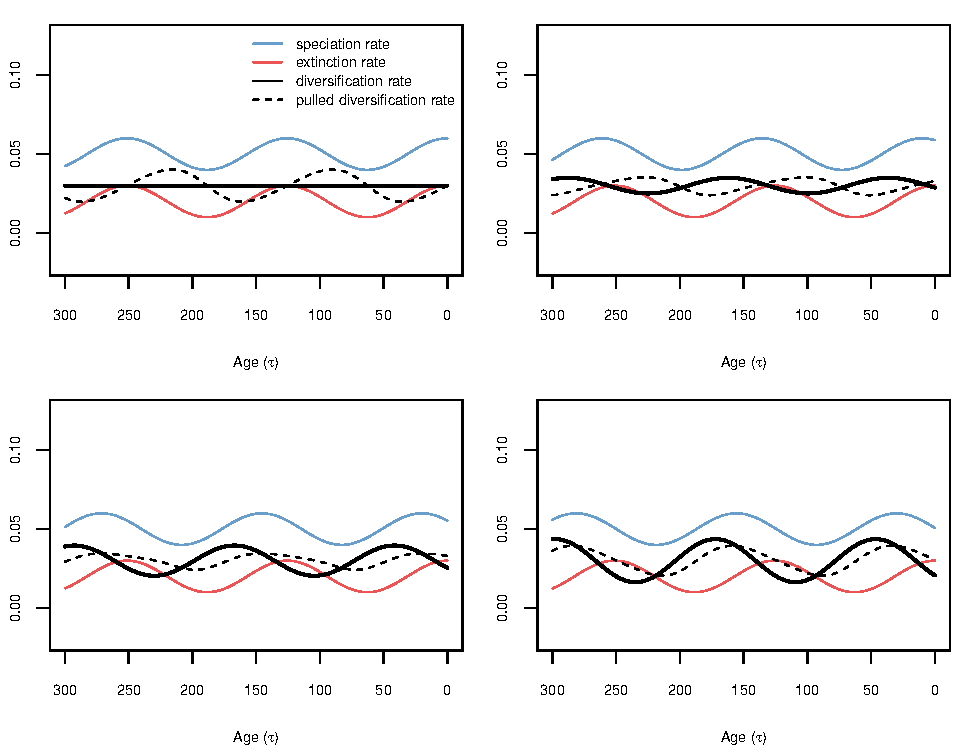
\includegraphics{supplement_files/figure-latex/unnamed-chunk-25-1.pdf}

\end{document}
